\documentclass[14pt, a4paper]{extarticle}

%\usepackage[T2A]{fontenc}
\usepackage[utf8]{inputenc} 
\usepackage[english,russian]{babel}
\usepackage{url}
%\usepackage{pscyr}

%\renewcommand{\rmdefault}{ftm}
\usepackage{setspace}
\onehalfspacing

\usepackage{changepage}
\usepackage{indentfirst} %первый абзац
\usepackage[noend]{algorithmic}
\usepackage{amssymb, amsmath, multicol,amsthm}
\usepackage{tabularx}
\usepackage{enumitem, multicol}
\usepackage{titleps,lipsum}
\usepackage{mathrsfs}
\usepackage{verbatim}
\usepackage{pb-diagram}
\usepackage{graphicx}
\graphicspath{ {images/} }
\usepackage{wrapfig}
\usepackage{xcolor}
\definecolor{new}{RGB}{255,184,92}
\definecolor{news}{RGB}{112,112,112}
\usepackage{wallpaper}
\usepackage{float}
\usepackage{hyperref}
\usepackage{multirow}
\usepackage{longtable}
\usepackage{rotating} 
\usepackage{epsfig}
\usepackage{subfig}
\hypersetup{
	linkbordercolor=new,
}


\allowdisplaybreaks
%\usepackage{geometry}
%\geometry{top=3cm,bottom=2cm,left=2cm,right=2cm}

\usepackage[margin=2cm,left=3cm,right=1.5cm]{geometry}


\binoppenalty=5000
\parindent=1cm

\renewcommand{\div}{\operatorname{div}}
\newcommand{\grad}{\operatorname{grad}}
\newcommand{\rot}{\operatorname{rot}}
\newcommand{\const}{\operatorname{const}}
\newcommand{\diag}{\operatorname{diag}}
\renewcommand{\leq}{\leqslant}
\renewcommand{\geq}{\geqslant}
\newtheorem{Lemma}{Лемма}
\def\proofname{Доказательство}
\newcommand{\anonsection}[1]{\section*{#1}\addcontentsline{toc}{section}{#1}}


\begin{document}
	
	\vskip 3mm
	
	\setcounter{page}{1}
	%%%%%%%% титульный лист %%%%%%%%%%%%%%%%%%%%%%%%%%%%%%%%%
	\begin{center}
		\thispagestyle{empty}
		
		{ Министерство общего и профессионального образования \\}
		{ Российской Федерации \\}
		
		
		
		{ Московский Физико-технический институт \\}
		
		{(Государственный университет) \\}
		
		{ Факультет управления и прикладной математики \\}
		
		{ Кафедра Acronis \\[4cm]}
		
		{ \bf \Large Выпускная квалификационная работа\\}
		
		{ \bf \Large{"Поиск аномалий во временных рядах системы Acronis Storage"\\[1cm]} }
		
		{\bf {Студента 4-го курса Угнивенко Виталия Алексеевича}\\[3cm]}
		
	\end{center}
	
	\begin{flushright}
		\bf{Научный руководитель}\\
		\bf{Андрей Кулага}\\[4cm]
	\end{flushright}
	
	\begin{center}
		Москва, 2020
	\end{center}
	
	\newpage
	\anonsection{Аннотация}
	\sectionmark{Аннотация}	
	
	Данная работа посвящена проблеме детектирования аномалий во    временных рядах, которая заключается в идентификации и обработке аномальных участков в потоках данных, получаемых из системы Acronis Storage. В результате работы была создана система поиска аномалий, главными преимуществами которой являются высокая точность и корректная работа на всём многообразии хранилищ данных компании Acronis.
	
	Выявление аномального поведения в автоматическом режиме позволит повысить  качество работы системы Acronis Storage, а также поможет предотвращать нештатные ситуации на этапах их зарождения. В этом и заключается актуальность проведения работы в данной области.
	
	\newpage
	\tableofcontents
	
	\newpage	
	\section{Введение}
	\sectionmark{Введение}
	Реалии современного мира вынуждают IT компании создавать всё более функциональные, но при этом и более технически сложные продукты. Очевидно, что с ростом глубины системы, уменьшается возможность прокрыть и обработать все возможные ситуации, потенциально ведущие к отклонению поведения данной системы от нормального.
	
	В свою очередь любые сбои в работе сложных технологических систем могут привести к существенным потерям, как со стороны компании, так и со стороны пользователей. Вот почему задача детектирования сбоев работы и анализа состояния системы в реальном времени всегда останется актуальной.
	
	Данная проблема касается и Acronis Storage, ведь это один из ключевых продуктов компании Acronis. Миллионы клиентов предпочли его для хранения, а также восстановления данных. Для предоставления своих услуг в этой области компания Acronis имеет десятки хранилищ данных. 
	
	Любые непредвиденные происшествия со стороны хранилищ данных могут привести к серьёзным проблемам, таким как выход из строя сервисов компании или потеря пользовательских данных, поэтому задача мониторинга работы систем и своевременного предупреждения сбоев в их работе становится крайне важной. 
	
	Учитывая количество информации, поступающей из хранилищ данных, остро встаёт вопрос об автоматизации этих процессов. Стандартными подходами к проблеме такого рода являются методы машинного обучения и анализ данных. Эти области современной науки позволяют нам построить автоматическую систему поиска аномалий в работе хранилищ данных, способную выявлять сложные шаблоны сбоев на ранней стадии их появления, тем самым заметно снижая сопутствующий ущерб. 
	
	Несмотря на то, что большое количество исследований на эту тему уже  было проведено, финальный алгоритм должен учитывать интересующие нас систему и данные.

	\newpage
	\subsection{План работы}
	Данная работа организована следующим образом 
	\begin{itemize}
	\item В \textbf{Главе 2} описывается, с данными какого рода мы имеем дело и что именно мы в этих данных хотим отыскать. 
	\item В \textbf{Главе 3} рассматривается, какая часть всех данных была выбрана для построения модели, а также причины этого выбора. 
	\item В \textbf{Главе 4} обсуждаются используемые методы предобработки данных, необходимые для создания качественной системы детектирования аномального поведения. 
	\item В \textbf{Главе 5} приводится описание предиктивной модели.
	\item В \textbf{Главе 6} описывается алгоритм распознавания аномалий во временных рядах.
	\item В \textbf{Главе 7} рассматриваются результаты поиска.
	\item В \textbf{Главе 8} приводятся примеры найденных аномалий.
	\item В \textbf{Главе 9} доказывается корректность предложенного алгоритма.
	\end{itemize}

	\newpage
	\section{Постановка задачи}
	\sectionmark{Постановка задачи}	
	\subsection{Данные}
	Информацию о функционировании хранилищ данных компании Acronis мы получаем, анализируя временные ряды метрик системы Acronis Storage, полученные нами при помощи системы Promoteus \cite{cite1}. 
	
	Временной ряд $X = \{x(t)|1 \leq t \leq m\}$ - это последовательность векторов-наблюдений $x(t) = (x_1(t), x_2(t), \dots x_d(t)) \in \mathbb {R}^d $ упорядоченных во времени. Чаще всего эти наблюдения собираются  через равные промежутки времени. Эти ряды  называются одноменрными временными рядами, если $d = 1$, и, соответственно,  многомерными, если $d \geq 2$.  
	
	Есть две основные цели анализа временных рядов:
 \begin{enumerate}
	 	\item \texttt{Изучение природы данных}
		 \item \texttt{Прогнозирование - предсказание его будущих значений по \\ прошлым или настоящим значениям, где время является \\ независимой переменной}
	 \end{enumerate}\label{list_of_metrics}
	 
	 Основное предположение в анализе временных рядов состоит в том, что некоторые шаблоны из прошлого будут появляться и в будущем. Как следствие, информация, полученная из анализа временных рядов может быть применена для прогнозирования, поиска аномалий и других приложений \cite{cite2}.  
	 	
	\subsection{Понятие аномальности}
	 Аномалия - это любое отклонение от стандартного поведения системы. На сегодняшний день существует большое количество работ по детектированию аномалий \cite{cite3}, в большей части которых используются методы идентификации отдельных объектов, которые отличаются от типичных объектов, но не учитывается аспект последовательности данных. Строго говоря аномалии подразделяют на 3 основных типа:
	 
	 \textbf{Точечная аномалия} - единичный экземпляр данных рассматривается как аномальный по отношению к остальным. На рис.1 экземпляры $A1$ и $A2$ являются аномальными по отношению к экземплярам $C1$ и $C2$.
	\begin{figure}[H]
		\centerline{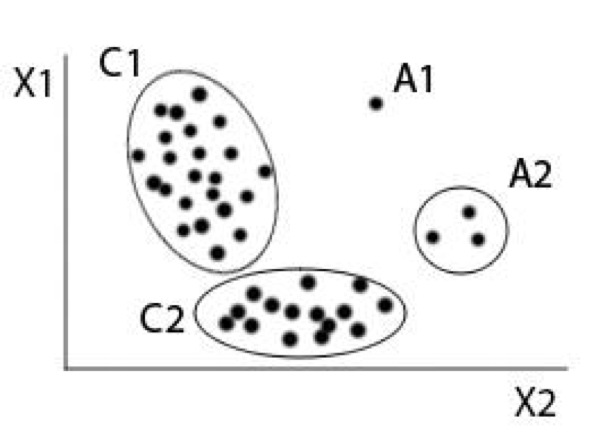
\epsfig{file=figures/anomaly_type1.png, scale=0.65}} 
		\caption{Пример точечных аномалий}
	\end{figure} 	
	
	 \textbf{Контекстуальная аномалия} - экземпляр данных рассматривается как аномальный в контексте. Для детектирования  данных аномалий необходимы контекстуальные и поведенческие признаки.  Во временных рядах  контекстуальный признак - время. А поведенческие признаки - любые признаки, которые описывают экземпляр данных без оглядки на контекст. Таким образом  отклонение от стандартного поведения системы определяется поведенческими признаками в контексте, определяемым контекстуальными признаками. Например на рис.2 точка $A$  - аномалия, при этом  точки $N_1, \dots, N_5$ - таковыми не являются. 
	
	 \textbf{Коллективные аномалии} -	последовательность элементов  является аномальной по отношению ко всему набору данных. То есть один элемент последовательности может являться аномалией, но одновременное появление таких элементов считается коллективной аномалией. 
	\begin{figure}[!htb]
		\minipage{0.49\textwidth}
		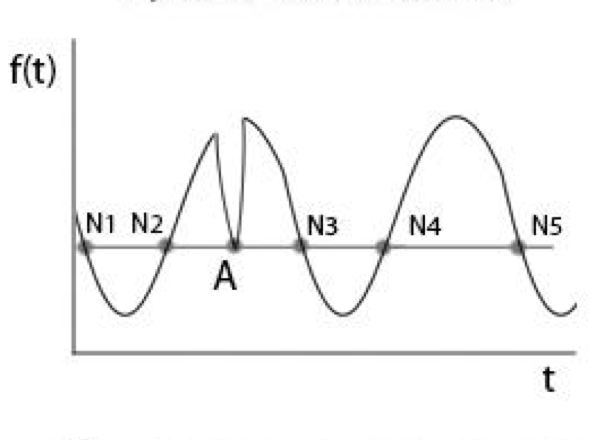
\includegraphics[width=\linewidth]{figures/anomaly_type2.png}
		\caption{Пример контекстуальной \\аномалии}
		\endminipage\hfill
		\minipage{0.49\textwidth}
		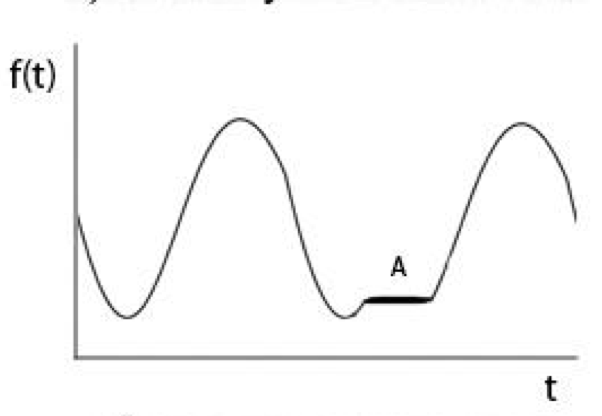
\includegraphics[width=\linewidth]{figures/anomaly_type3.png}
		\caption{Пример коллективных\\ аномалий}
		\endminipage
	\end{figure}
	
	\section{Отбор данных}
	\sectionmark{Отбор данных}	
	Чтобы покрыть максимальное количество шаблонов поведения системы с учётом высокой трудоёмкости вычислений, были использованы данные за полгода со следующих хранилищ:
	\begin{enumerate}
	 	\item \texttt{au2-acs1}
	 	\item \texttt{us6-acs2}
	 	\item \texttt{eu3-acs1}
	 	\item \texttt{us3}
	 \end{enumerate}\label{list_of_dc}
	
	Детальный анализ временных рядов, описывающих работу системы, привёл к выводу о необходимости анализа временных рядов abgw, ввиду их интерперитуемости и широкого использования всеми хранилищами данных. В качестве целевой переменной была выбрана следующая метрика:
	$$\texttt{sum(abgw\_req\_latency\_ms\_sum\{req $\in$ \{"OpenFile"\\, "Append" \}\})}$$
	Выбор обусловлен тем, чем смысл данной метрики - суммарная задержка исполнения соответствующих операций. По мнению экспертов, аномальное поведение системы зачастую сопровождается скачком задержки исполнения данных операций.  Обзор остальных метрик привел нас к выбору наиболее информативных:
	 \begin{enumerate}
	 	\item \texttt{sum(abgw\_req\_latency\_ms\_count\{req = "OpenFile"+ "Append" \})} 
	 	\item \texttt{abgw\_iop\_latency\_ms\_count\_open(pcs)}
	 	\item \texttt{abgw\_iop\_latency\_ms\_sum\_open(pcs)}
	 	\item \texttt{abgw\_conns}
	 	\item \texttt{abgw\_account\_lookup\_errs\_total\{err="OK"\}}
	 	\item \texttt{abgw\_account\_pull\_errs\_total\{err="OK"\}}
	    \item \texttt{abgw\_accounts}
	 	\item \texttt{abgw\_append\_throttle\_delay\_ms\_total}
	 	\item \texttt{abgw\_fds}
	 	\item \texttt{abgw\_file\_lookup\_errs\_total\{err="OK"\}}
	 	\item \texttt{abgw\_files}
	 	\item \texttt{abgw\_read\_bufs}
	 	\item \texttt{abgw\_read\_bufs\_bytes}	
	 	\item \texttt{abgw\_read\_bytes\_total\{proxied="0"\}}	
	 	\item \texttt{abgw\_read\_reqs\_total}	
	 \end{enumerate}\label{list_of_metrics}
	
	\section{Предобработка данных}
	\sectionmark{Предобработка данных}	
		
	Основные составляющие любого временного ряда
	\begin{itemize}
	\item Тренд - это плавное долгосрочное изменение уровня ряда в плане возрастания или убывания значений. 
	\item Сезонность - циклические изменения уровня ряда с постоянным периодом.
	\item Цикл - изменение уровня ряда с переменным периодом. 
	\item Ошибка - непрогнозируемая случайная компонента ряда. В идеале - нормальная центрированная случайная величина.
	\end{itemize}
	
	Стационарность – постоянство характеристик процесса со временем, таким образом стационарный временной ряд лишён сезонной и трендовой составляющей. По теореме Вольда любой стационарный ряд может быть описан моделью ARMA(p, q) с любой точностью. Именно поэтому остро стоит вопрос о поиске универсального метода предобработки временных рядов для всего многообразия хранилищ данных системы Acronis Storage.
	\subsection{Тренд}
	\begin{figure}[H]
		\centerline{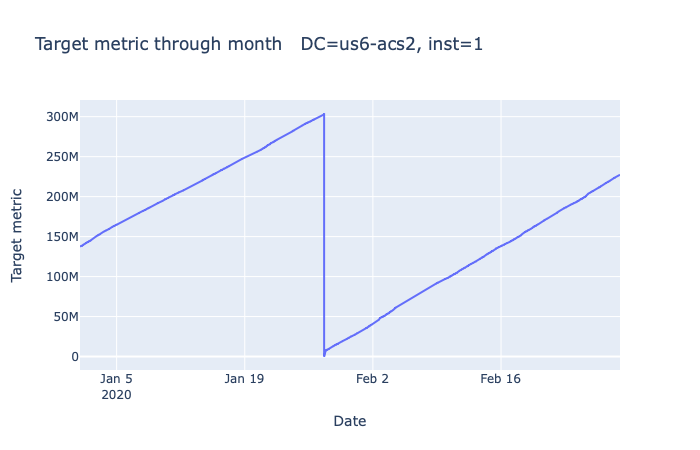
\epsfig{file=figures/target_metric.png, scale=0.5}} 
		\caption{Целевая метрика за исследуемый период}
		\label{target_metric_fig1}
	\end{figure} 
	
	Если не брать во внимание резкий скачок целевой переменной вниз, обусловленный перезагрузкой системы, то легко заметить, что у нашей целевой переменной есть тренд к возрастанию, от которого можно избавиться путём перехода к приращениям первого порядка. Перейдём в пространство производных и уберём данные, соответствующие перезагрузке. 
	
	\begin{figure}[H]
		\centerline{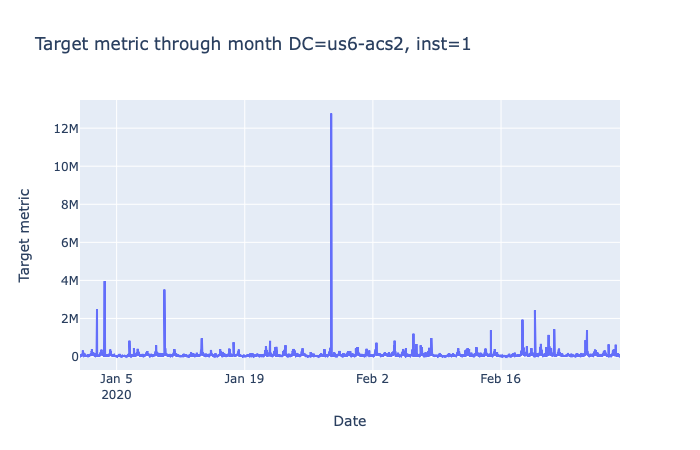
\epsfig{file=figures/target_derivative.png, scale=0.5}} 
		\caption{Целевая метрика в пространстве производных за исследуемый \\ период}
		\label{target_metric_fig1}
	\end{figure} 	
	
	У полученной переменной существует простая интерпретация - приращение суммарной задержки, другими словами задержка, накопленная за одну минуту.
	
	\subsection{Сезонность}
	  Если посмотреть на Рис. 6 (часть Рис. 5), то можно заметить, что нашему временному ряду присуща дневная сезонность. Но дискретность данных высока, поэтому избавиться от сезонности с помощью сезонного дифференцирования не удаётся. 
	 
	 \begin{figure}[H]
		\centerline{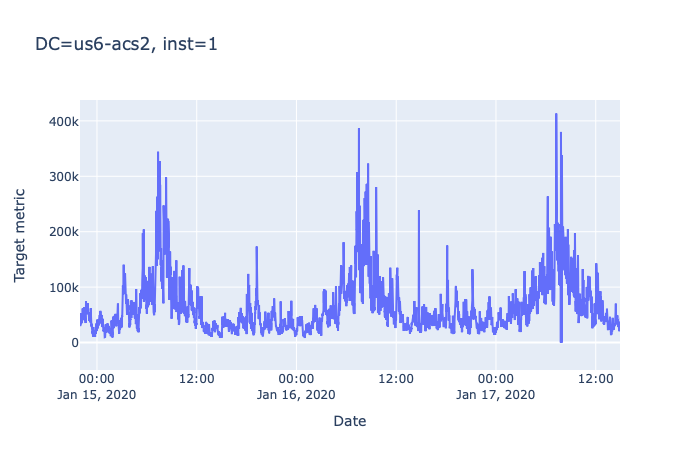
\epsfig{file=figures/target_seasonality.png, scale=0.5}} 
		\caption{Целевая метрика в пространстве производных}
		\label{target_metric_fig1}
	\end{figure} 	
	
	\subsection{Масштабирование}	
	Необходимость в масштабировании заключена в следующем: градиентный спуск прекрасно работает, если линии уровня функции походят на окружности, так как какая бы не была начальная точка, вектор антиградиента будет направлен точно в сторону минимума функции, а итеративный процесс будет сходиться быстро. А если линии уровня функции имеют эллипсоидный вид, другими словами признаки имеют разный масштаб, то направление вектора антиградиента будет слабо совпадать с направлением в сторону минимума функции. Как следствие, градиентный спуск будет делать много шагов и  сходимость итеративного процесса будет медленная. Более того, существует риск расхождения процесса при неверно подобранном размере шага.
	\begin{figure}[H]
		\centerline{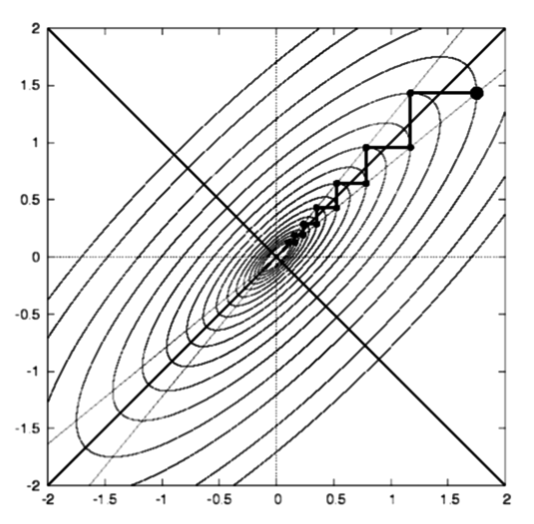
\epsfig{file=figures/scaling.png, scale=0.55}} 
		\caption{Градиентный спуск без масштабирования}
		\label{target_metric_fig1}
	\end{figure} 	
	 
	 Используем масштабирование на отрезок $[0, 1]$. Для этого необходимо вычислить максимальное и минимальное значение каждого признака на обучающей выборке:
	  $$m_j = min(x_1^j, \dots, x_l^j)$$
	  $$M_j = max(x_1^j, \dots, x_l^j)$$
	 
	 Тогда значение каждого признака на конкретном объекте преобразовывается следующим образом:
	 $$x_i^j := \dfrac{x_i^j - m_j}{M_j-m_j}$$
	\subsection{Удаление участков с перезагрузками}	
	Во время перезагрузок системы целевая переменная в пространстве производных принимает большие по модулю отрицательные значения. Перезагрузка - это не стабильное состояние, обучаться на таких интервалах нет смысла, поэтому мы убираем их из обучающей выборки.	
	\section{Модель прогнозирования временного ряда}	
	\subsection{Введение в линейную регрессию}	
	Линейный алгоритм в задаче регрессии выглядит следующим образом:
	$$a(x) = w_0 + \sum_{j=1}^{d}w_j \cdot x^j,$$ 
	где $w_0$ — свободный коэффициент, $x^j$ - признаки, описывающие объект $x$, а $w_j$ — соответствующие веса. Если добавить $(d+1)-$ый признак, принимающий на каждом объекте значение $1$, линейную алгоритм может быть переписан в следующем виде: 
	$$a(x) = \sum_{j=1}^{d+1}w_j \cdot x^j = (w,x),$$ 
	где $(w,x)$ - скалярное произведение векторов. В качестве меры ошибки можно выбрать отклонения от предсказания: $|a(x)-y|$. Но данная функция не является гладкой, следовательно мы не сможем легко использовать градиентные методы для оптимизации данного функционала. Лучше в качестве меры ошибки выбрать квадрат отклонения от прогноза: $(a(x)-y)^2$
	
	А функционал ошибки, он же среднеквадратичная ошибка алгоритма, он же MSE, задаётся следующим образом:
	$$Q(a(x), X) = \dfrac{1}{l} \cdot \sum_{i=1}^{l} (a(x_i)- y_i)^2$$
	А так как функционал зависит только от вектора весов $w$, мы можем переписать в следующем виде:
	$$Q(w, X) = \dfrac{1}{l} \cdot \sum_{i=1}^{l} ((w,x_i)- y_i)^2$$
	Обучение модели линейной регрессии состоит в том, чтобы минимизировать функционал ошибки:
	$$Q(w, X) = \dfrac{1}{l} \cdot \sum_{i=1}^{l} ((w,x_i)- y_i)^2\longrightarrow \min_{w}$$
	Перепишем в матричной форме. Пусть $y = (y_1, \dots, y_l)^T $- вектор ответов. А матрица $X$ состоит из описаний объектов из обучающей выборки:
	$$X = 
\begin{pmatrix}
  x_{11} \dots x_{1d}\\
  \dots \dots \dots\\
  x_{l1} \dots x_{ld}
\end{pmatrix}
$$
Тогда задачу обучения можно записать следующим образом:
$$Q(w, X) = \dfrac{1}{l}||Xw-y||_2^2\longrightarrow \min_{w}$$

Заметим, что  среднеквадратическая ошибка - выпуклая и гладкая функция. Выпуклость гарантирует единственность  минимума, а гладкость - \\ существование вектора градиента в каждой точке. Поэтому для поиска решения используется метод градиентного спуска: 
$$w^0\in \mathcal {N}(0,1)$$
 $$w^t = w^{t-1}-\eta_t \nabla Q(w^{t-1},X)$$
$$||w^t-w^{t-1}||<\varepsilon$$
	\subsection{Использование модели линейной регрессии для прогнозирования временных рядов}	
	Предложенная предиктивная модель является логическим усовершенствованием модели  ARIMA(p, d, q).  
	
	ARIMA(p, d, q) - интегрированная модель авторегресси - скользящего среднего, которая  представляет из себя  расширение модели ARMA(p, q) для нестационарных временных рядов. Иначе говоря, разности нестационарного временного ряда порядка d описываются моделью ARMA(p, q). \\\\В свою очередь, модель ARMA(p, q) состоит из двух моделей:
	
	 AR(p) - значение временного ряда в настоящий момент времени линейным образом зависит от предыдущих p значений данного ряда.
	 
	  MA(q) - значение временного ряда в настоящий момент времени линейным образом зависит от предыдущих q значений ошибки модели.
	
	Как уже было сказано, от чтобы избавиться от нестационарности во временных рядах, был произведён переход к приращениям первого порядка, таким образом мы используем модель ARIMA(p, d, q) c d = 1. Таким образом в новом признаковом пространстве модель ARIMA(p, 1, q) выглядит следующим образом: \\
 $$y_t = \varepsilon_t+ \sum_{i=1}^{p}\alpha_i \cdot y_{t-i} + \sum_{i=1}^{q}\beta_i \cdot \varepsilon_{t-i}$$
 
$\{\varepsilon _{t}\}$ - независимые и одинаково распределённые случайные величины, с нулевым средним - белый шум, а $\alpha _{1},\dots ,\alpha _{p}$ и $\beta _{1},\ldots ,\beta _{q}$ - авторегрессионные коэффициенты и коэффициенты скользящего среднего. Поскольку ошибку наблюдать невозможно, значения $\{\varepsilon_t\}$ из прошлого  заменяются на остатки, а из будущего заменяются на нули , так как ошибка в среднем ноль. Поэтому предсказание можно записать следующим образом: 
$$\hat{y_t} = \sum_{i=1}^{p}\alpha_i \cdot y_{t-i} + \sum_{i=1}^{q}\beta_i \cdot \hat{\varepsilon_{t-i}}$$

Так вот остатки хорошей предиктивной модели должны обладать следующими свойствами:
 \begin{enumerate}
	 	\item \texttt{Несмещённость. Если остатки модели в среднем не равны \\нулю, то прогноз настолько плох, что если его сдвинуть \\на константу, то он станет лучше.}
	 	\item \texttt{Стационарность. Если её нет, то в остатках есть структура \\ и мы не смогли выбрать всю информацию из данных.}
	 	\item \texttt{Неавтокореллированность. Если остатки коррелированны, то \\они неслучайны и несут информацию, которую мы не смогли \\выбрать из данных.}
\end{enumerate}

Остатки подобранной классическими методами модели ARIMA(8,1,5) не удовлетворяли некоторым из этих свойств. Это значит, что класс моделей ARIMA(p, d, q) недостаточно богат, чтобы содержать в себе модель, хорошо описывающую целевую переменную. Поэтому для предсказания используем логическое усовершенствование модели  ARIMA(p, d, q) - в качестве признаков будем использовать не только целевую переменную и остатки модели, но и другие метрики, описывающие работу системы. Таким образом предиктивная модель имеет следующий вид:
$$\hat{y_t} = \sum_{i=1}^{p}\alpha_i \cdot y_{t-i} + \sum_{i=1}^{q}\beta_i \cdot \hat{\varepsilon}_{t-i} +\sum_{k=1}^{r}\sum_{i=1}^{p}\gamma_i x_{t-i}^{k}$$
Где $x_{t-i}^{k}$ - значение $k$-го признака в момент времени $(t-i)$. Таким образом, нам необходимо подобрать параметры $\{\alpha_i\}$, $\{\beta_i\}$ и $\{\gamma_i\}$ на обучении, а параметры p, q и r на валидации. 
\subsubsection{Отбор признаков}	
Построим самую простую линейную модель на всех рассматриваемых метриках. Так как мы используем MinMaxScaler, то веса при признаках-метриках равносильны их значимости. Тогда для каждой метрики посчитаем её суммарную по всем хранилищам данных значимость для модели.
\begin{figure}[H]
		\centerline{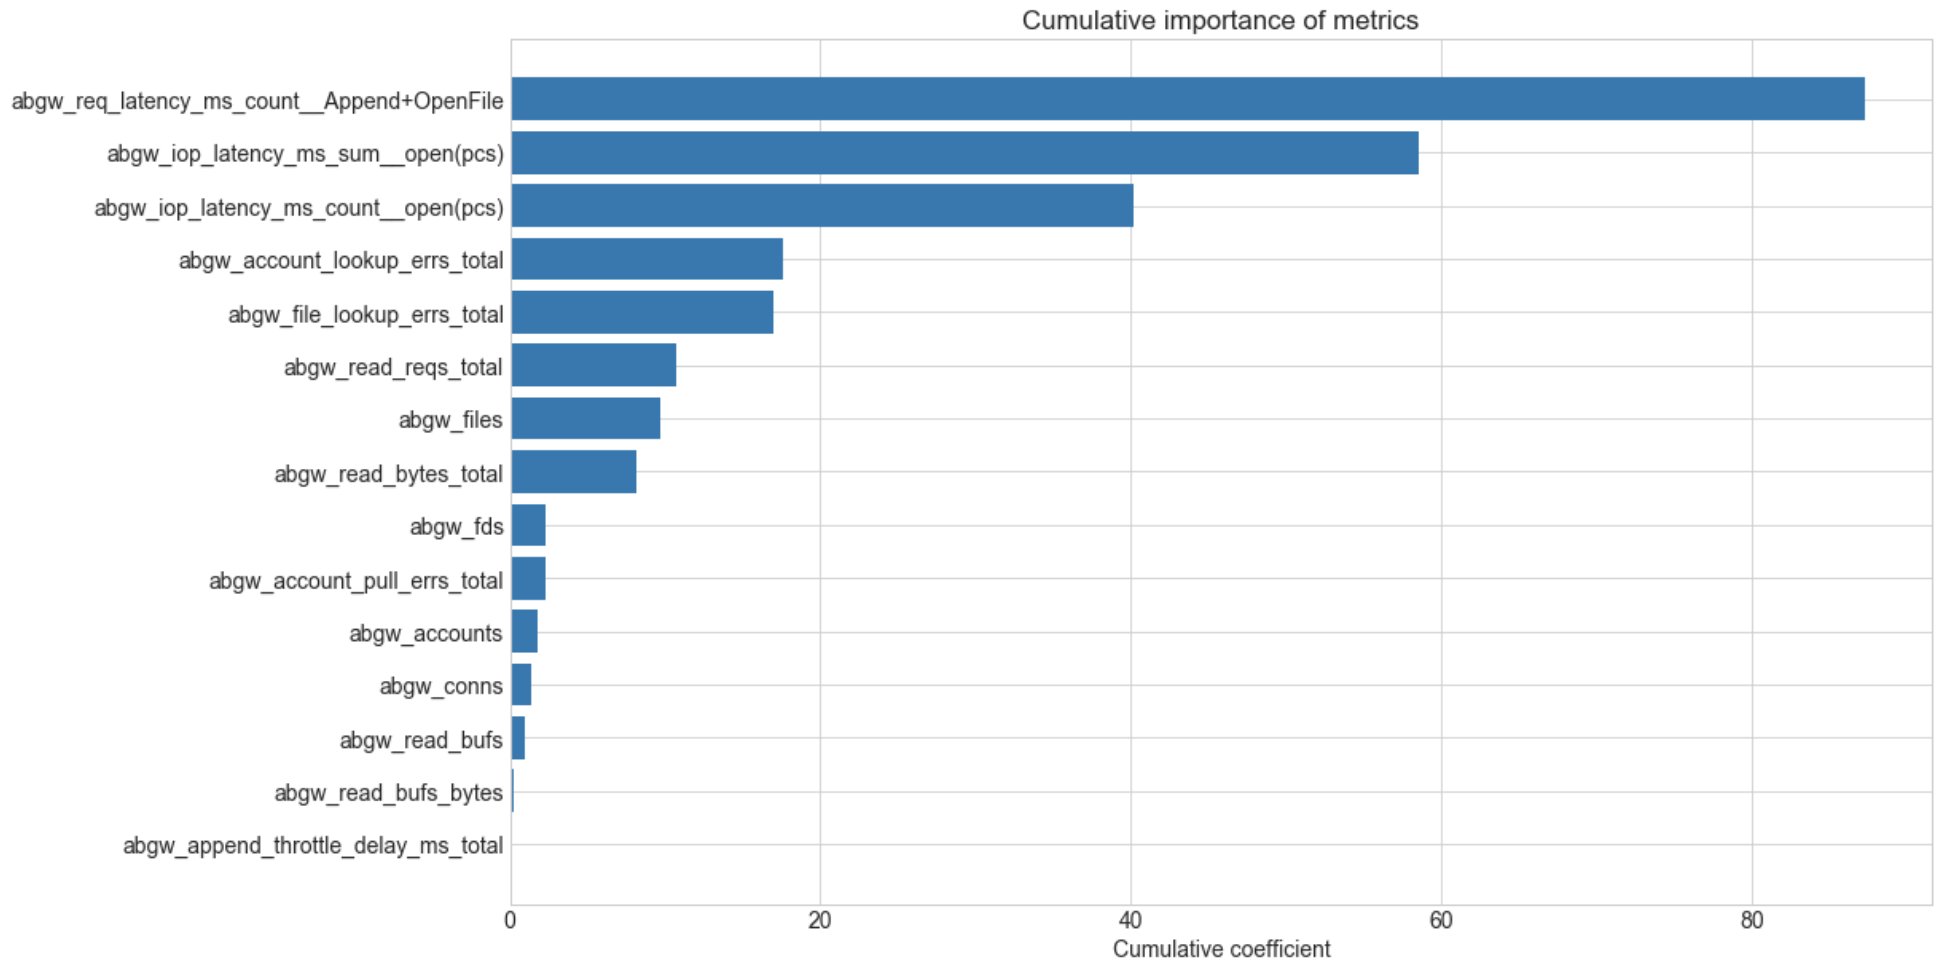
\epsfig{file=figures/feature_importance.png, scale=0.5}} 
		\caption{Cуммарная по всем хранилищам данных значимость метрик}
		\label{target_metric_fig1}
	\end{figure} 	
Посмотрим, как кумулятивная ошибка зависит от количества признаков в модели:
\begin{figure}[!htb]
		\minipage{0.49\textwidth}
		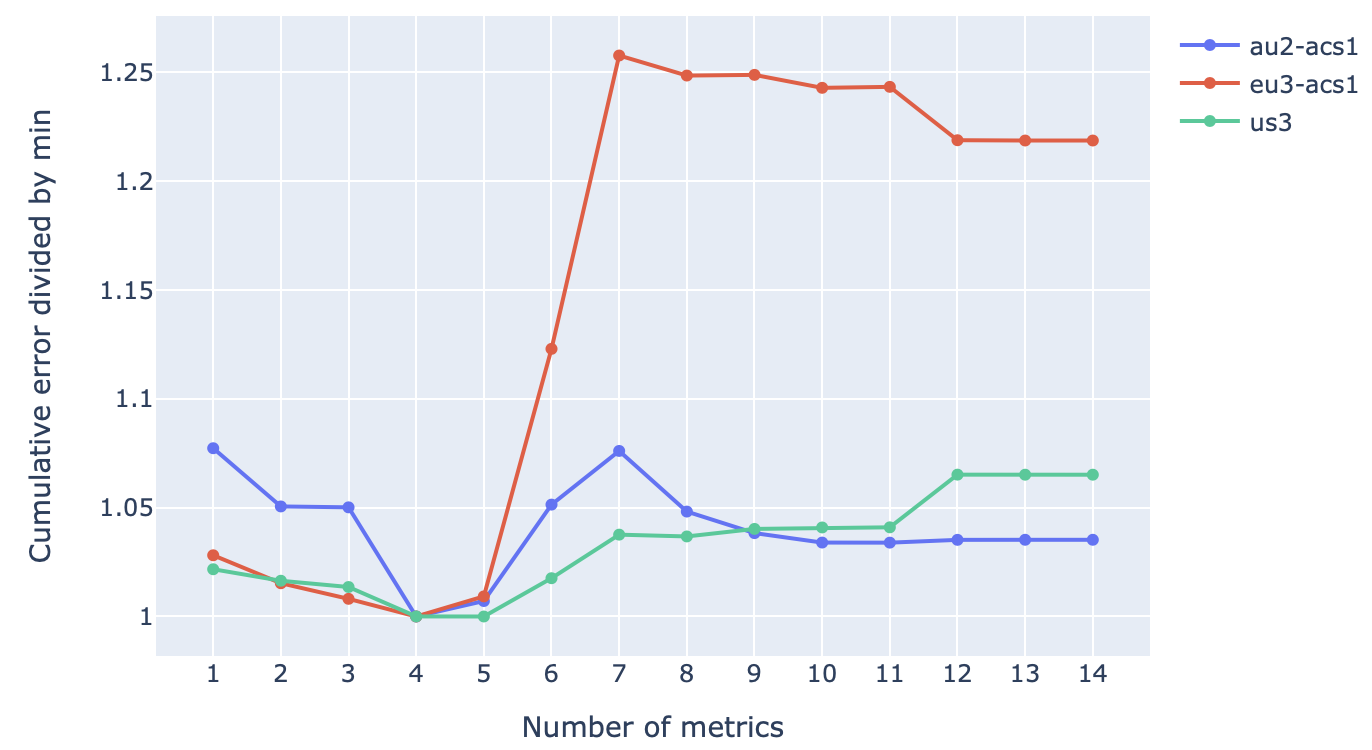
\includegraphics[width=\linewidth]{figures/mae_num_features_1.png}
		\caption{Кумулятивная ошибка  от \\количества признаков}
		\endminipage\hfill
		\minipage{0.49\textwidth}
		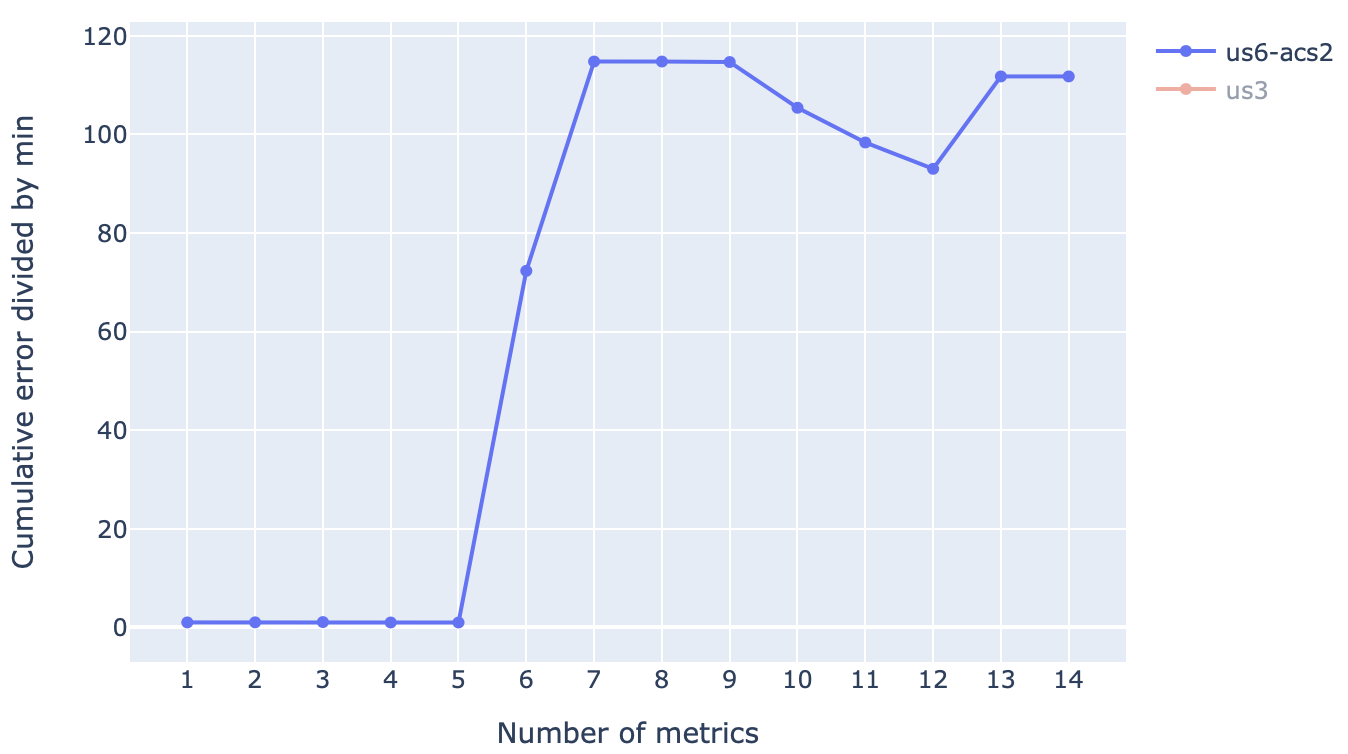
\includegraphics[width=\linewidth]{figures/mae_num_features_2.png}
		\caption{Кумулятивная ошибка  от \\количества признаков}
		\endminipage
	\end{figure}
	
Таким образом необходимо взять $r=5$ наиболее значимых метрик.

\subsubsection{Поиск оптимального количества задержек целевой переменной и признаков}	
Построим зависимость средней за минуту ошибки модели от количества задержек:
\begin{figure}[H]
		\centerline{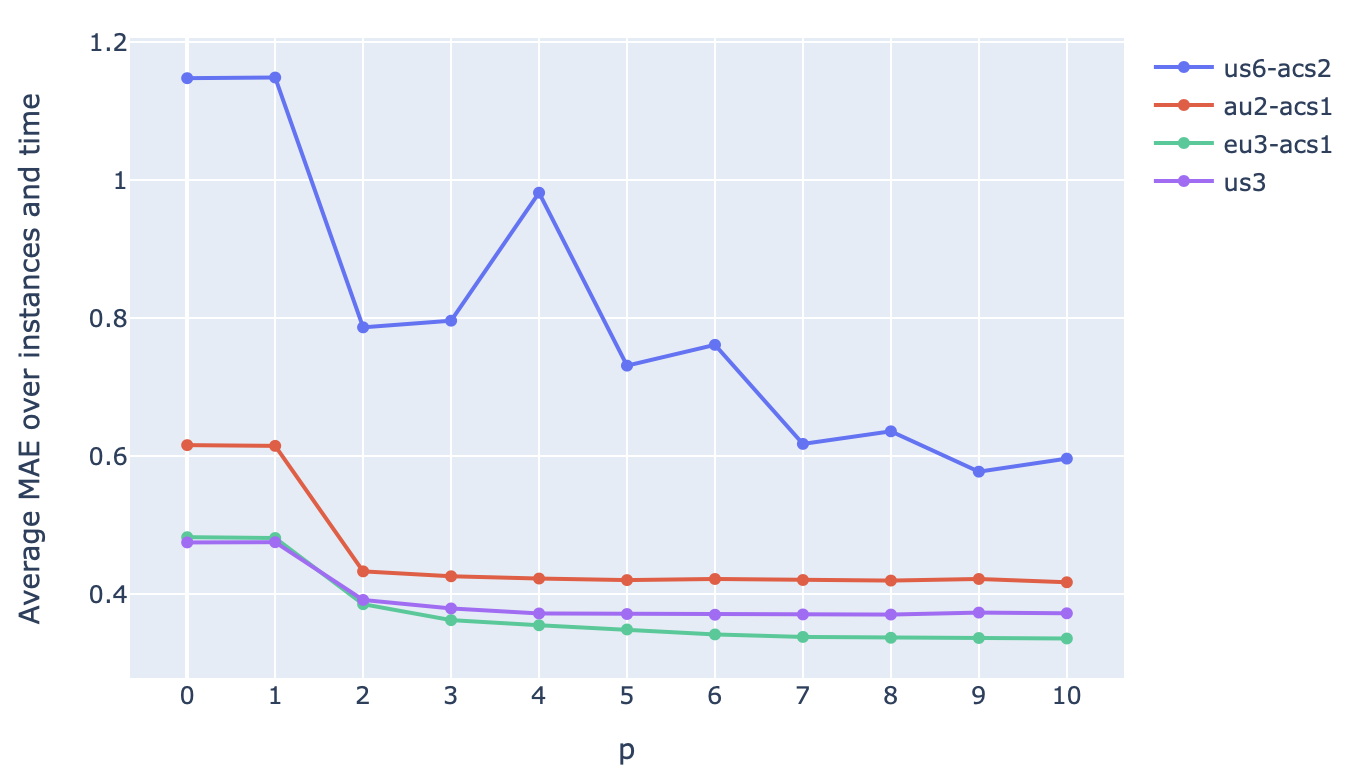
\epsfig{file=figures/avarage_mae_p.png, scale=0.5}} 
		\caption{Средняя за минуту ошибка модели от количества задержек}
		\label{target_metric_fig1}
	\end{figure} 	
Можно  сделать вывод, что необходимо взять $p = 2$, так как добавление большего числа задержек не приносит значительных улучшений, а лишь вносит дополнительный шум.

\subsubsection{Поиск оптимального количества задержек ошибки}	
Так как мы не можем наблюдать ошибку, то построим модель без  задержек ошибки, найдём остатки и построим модели с полученными  остатками в качестве задержек ошибки. Посмотрим на зависимость средней по экземплярам хранилища данных кумулятивной ошибки от количества задержек ошибки. 
\begin{figure}[H]
		\centerline{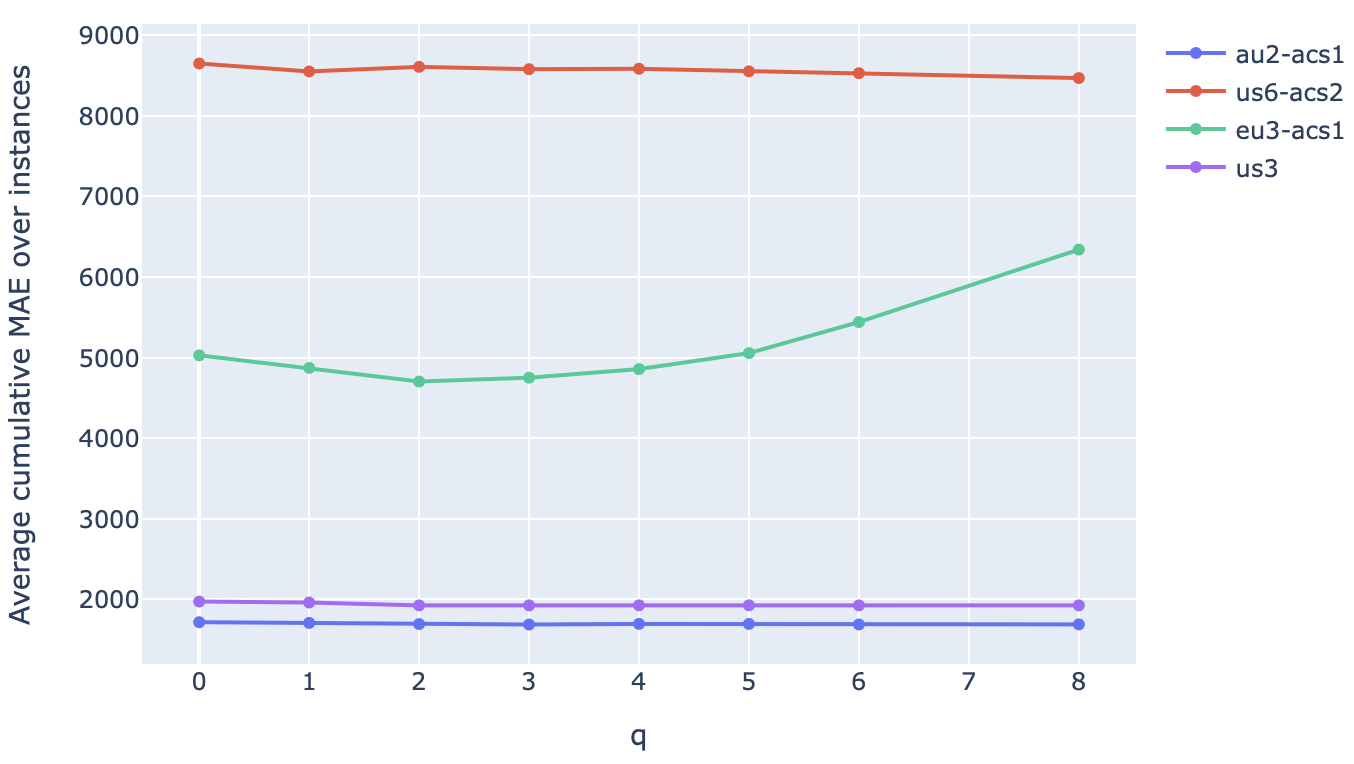
\epsfig{file=figures/q_for_error.png, scale=0.5}} 
		\caption{Средняя за минуту ошибка модели от количества задержек}
		\label{target_metric_fig1}
\end{figure} 	
Можно  сделать вывод, что необходимо взять $q = 2$, так как добавление большего числа задержек не приносит значительных улучшений, а лишь вносит дополнительный шум.
	
	\section{Поиск аномалий}	
	\subsection{ Алгоритм}	
	На основе имеющихся временных рядов и предсказаний нашей модели, создадим временные ряды, анализ которых и приведёт нас к обнаружению аномалий. Как уже было отмечено выше, смысл целевой переменной - суммарная задержка рассматриваемых процессов. Логично предположить, что среднее значение и дисперсия задержек процессов входят в число временных рядов, анализ которых даёт информацию о аномальности системы. Чтобы получить эти временные ряды, рассмотрим следующую метрику:\\ 
	$$\texttt{abgw\_iop\_latency\_ms\_bucket\{err="OK"\\, iop="pread"\\, proxied="0"\}}$$
	
	Данная метрика показывает, как много запросов (нарастающим итогом) в данный момент времени завершилось с задержкой менее, чем соотвествующее значение. Из неё получим метрику, содержащую информацию о количестве запросов, которые в данный момент времени завершились с задержкой в соответствующем диапазоне.
	\begin{figure}[!htb]
		\minipage{0.49\textwidth}
		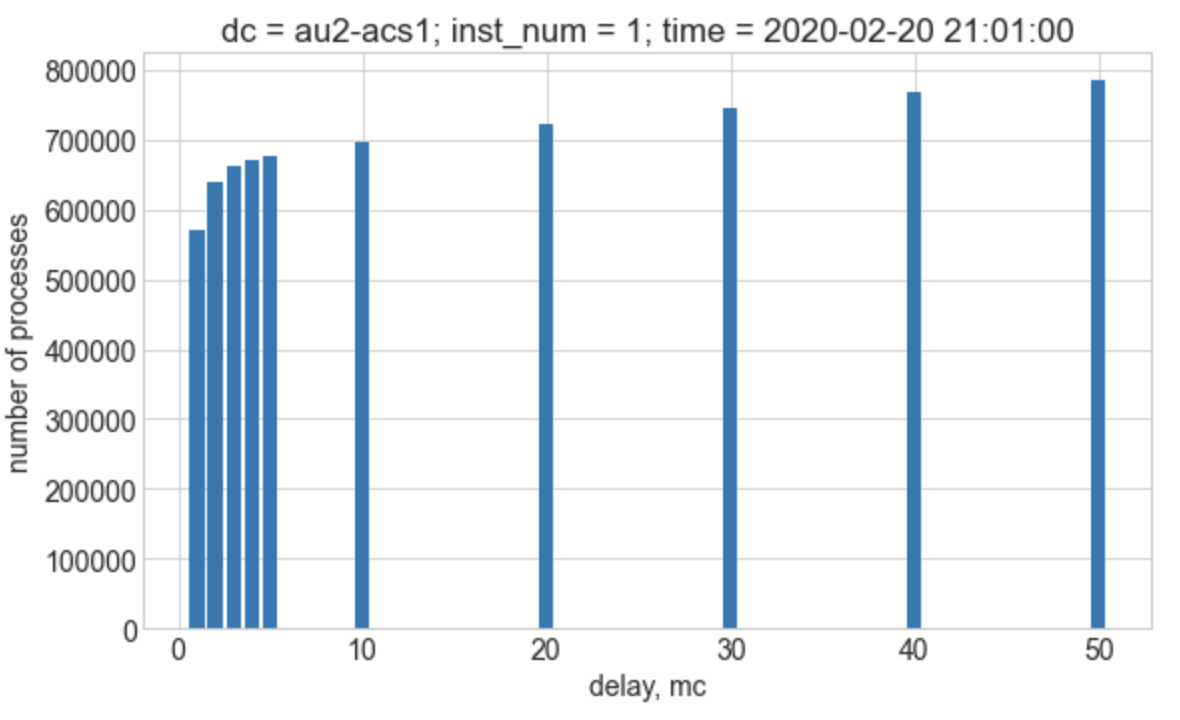
\includegraphics[width=\linewidth]{figures/delays_under_time.png}
		\caption{Количество запросов с задержкой менее, чем соответствующиие значения (нарастающим итогом).}
		\endminipage\hfill
		\minipage{0.49\textwidth}
		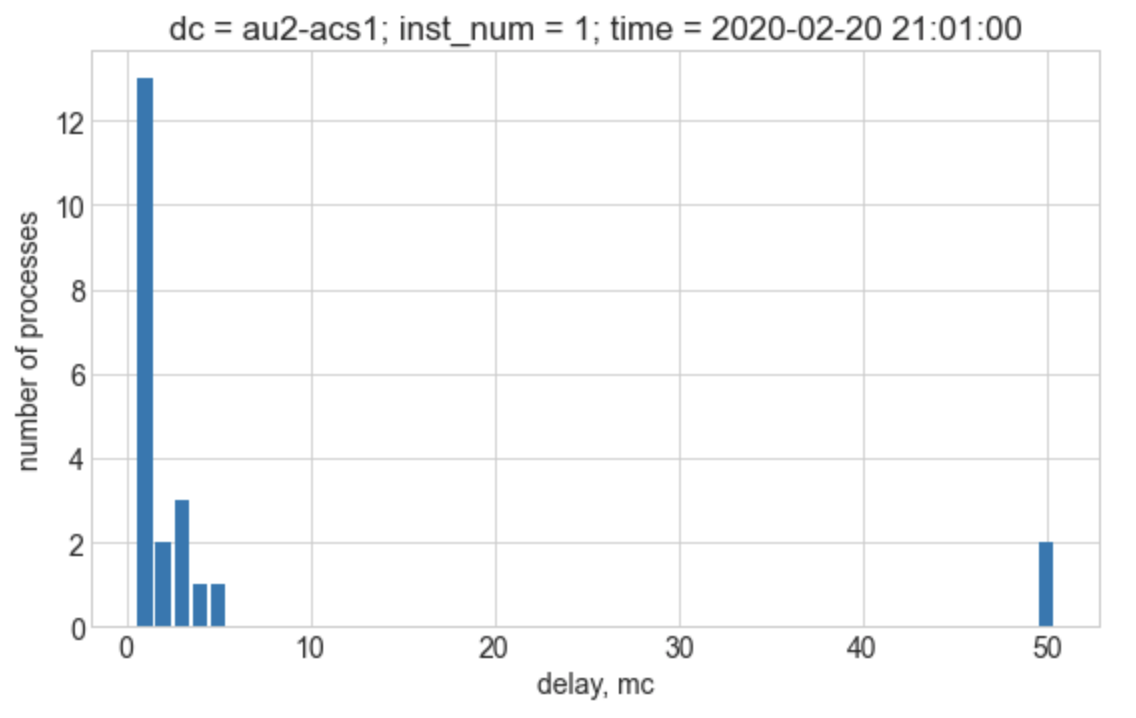
\includegraphics[width=\linewidth]{figures/delays_with_time.png}
		\caption{Количество запросов с задержкой в соответствующем диапазоне.}
		\endminipage
	\end{figure}
	
	 На основе этого находим выборочное среднее и дисперсию задержек запросов в каждый момент времени.
	 $$mean_k = \dfrac{1}{\mathbb {I}([0, \infty])} \cdot \sum _{i, j>i}\mathbb {I}([i, j]) \cdot \dfrac{j - i}{2} $$
	 $$variance_k = \dfrac{1}{\mathbb {I}([0, \infty])} \cdot \sum _{i, j>i}\mathbb {I}([i, j]) \cdot \left( \dfrac{j - i}{2} - mean_k\right) ^2 $$
	  где $\mathbb {I}([i, j])$ - количество запросов, задержка которых содержится в интервале от $i$ ms до  $ j$ ms. 
	 \begin{figure}[H]
		\centerline{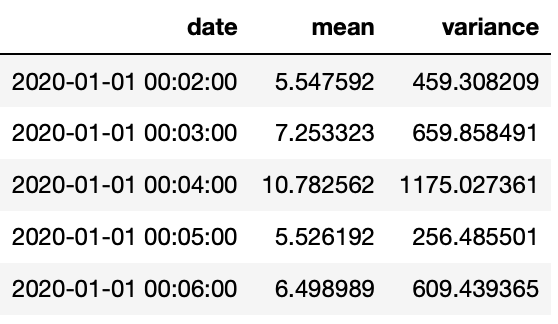
\epsfig{file=figures/table_maen_and_var.png, scale=0.9}} 
		\caption{Среднее значение и дисперсия задержки в каждый момент времени}
		\label{target_metric_fig1}
	\end{figure} 
	Предложенный алгоритм поиска аномалий опирается на предположение о нормальности среднего значения и дисперсии задержек запросов. Проверим эту гипотезу.
	\begin{figure}[!htb]
		\minipage{0.49\textwidth}
		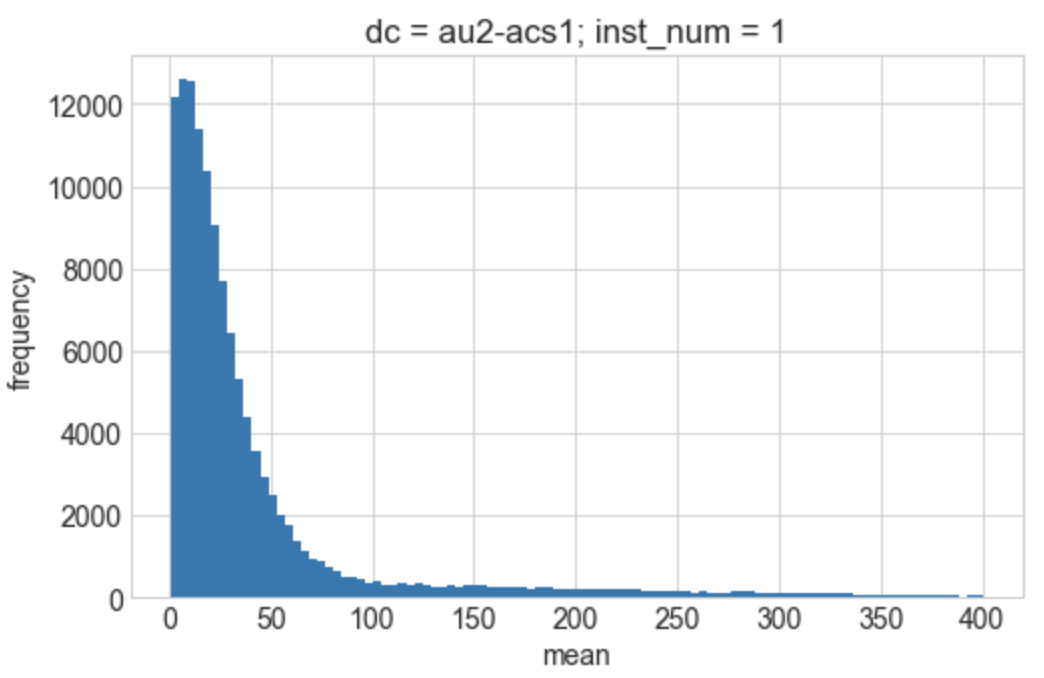
\includegraphics[width=\linewidth]{figures/mean_hist.png}
		\caption{Гистограмма среднего значения задержки}
		\endminipage\hfill
		\minipage{0.49\textwidth}
		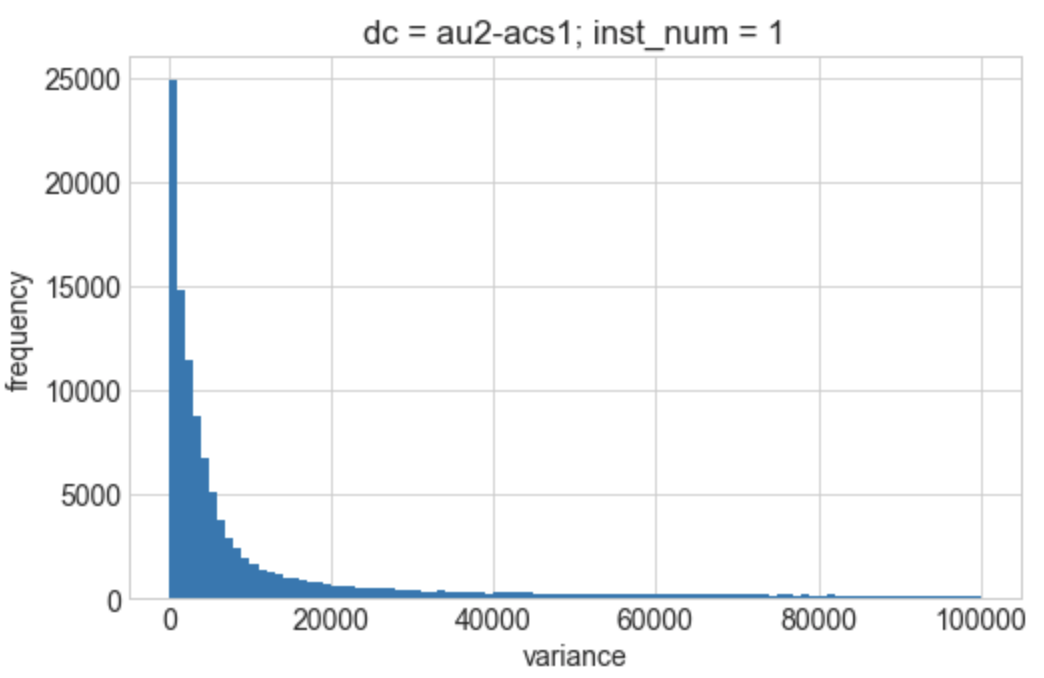
\includegraphics[width=\linewidth]{figures/variance_hist.png}
		\caption{Гистограмма дисперсии задержки}
		\endminipage
	\end{figure}
	
	Для визуальной проверки используем Q-Q plot. В статистике \\ Q-Q  plot - это график, который предоставляет графический метод для сравнения двух распределений путем построения их квантилей, где квантиль - это  значение, которое случайная величина не превышает с заданной вероятностью
	$$F_X(x_{\alpha})= \mathbb{P}(X \leq x_{\alpha})\geq\alpha$$
	Данные выборки сортируются в порядке возрастания, а затем наносятся на график в сравнении с квантилями, рассчитанными из теоретического распределения. Таким образом, получившаяся кривая является параметрической кривой с параметром, который является номером интервала для квантиля. Если распределения линейно связаны, то точки на графике будут приблизительно лежать на линии. Данный метод просто визуальная проверка, а не строгое доказательство, но он позволяет нам сразу увидеть, является ли наше предположение правдоподобным или нет.
	\begin{figure}[!htb]
		\minipage{0.49\textwidth}
		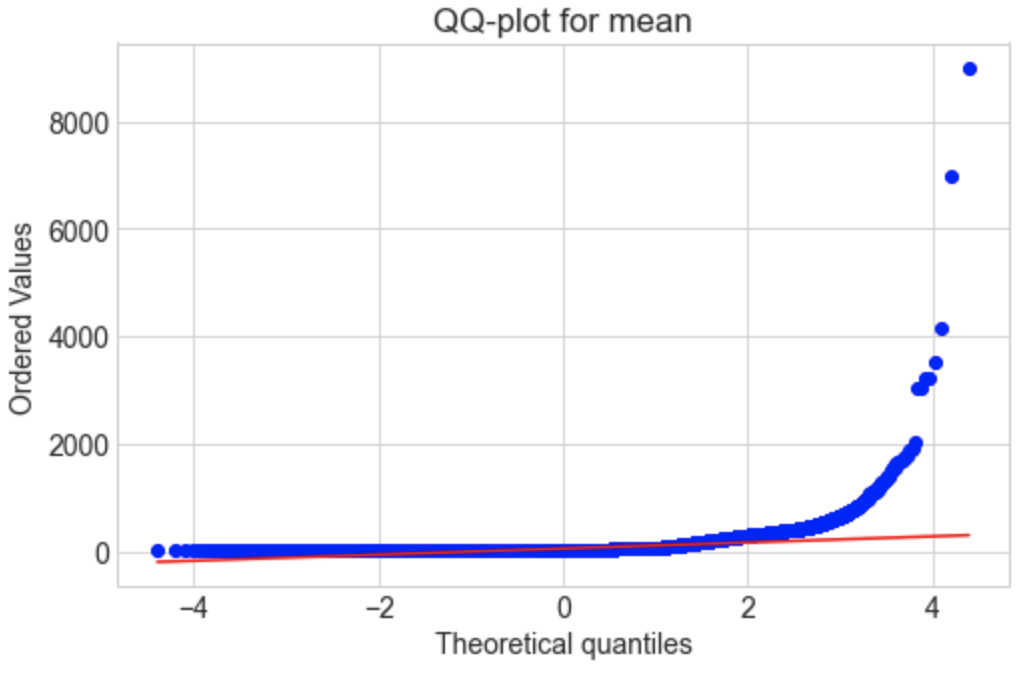
\includegraphics[width=\linewidth]{figures/qq_mean.png}
		\caption{dc = au2-acs1; inst = 1}
		\endminipage\hfill
		\minipage{0.49\textwidth}
		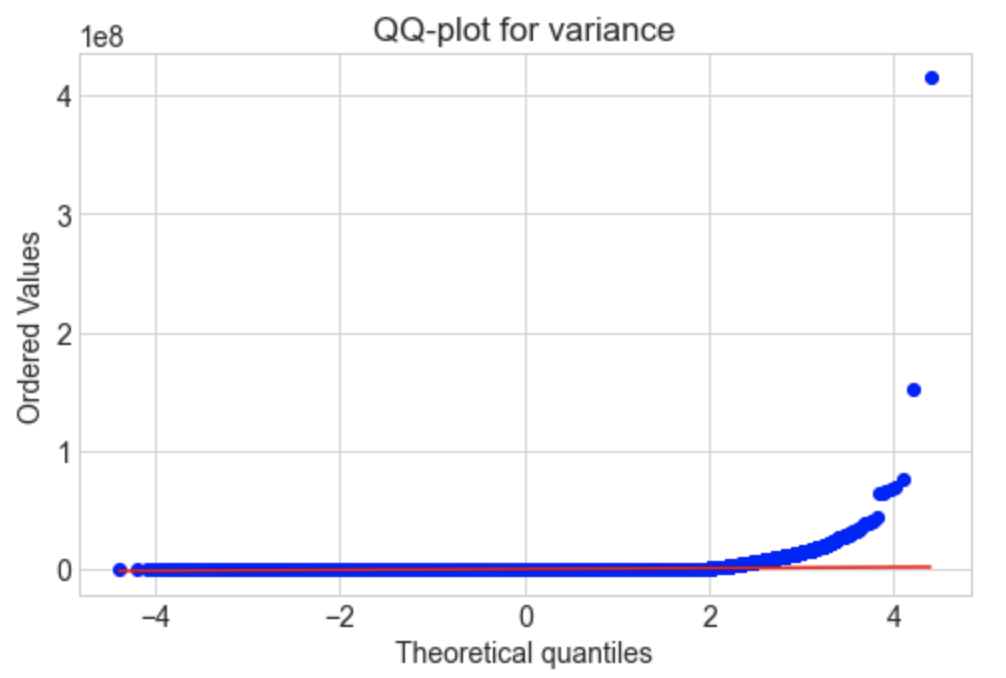
\includegraphics[width=\linewidth]{figures/qq_variance.png}
		\caption{dc = au2-acs1; inst = 1}
		\endminipage
	\end{figure}
	
	Из графиков можно сделать вывод о том, что наше предположение правдоподобно, так как большая часть данных действительно лежит на прямой. Более того, не лежащие на прямой точки являются потенциально аномальными.
	\\
	
	Проверим наше предположение с помощью критерия Харке-Бера:
	\\Выборка: $X^n$
	\\Нулевая гипотеза: $H_0: X\sim\mathcal {N}(\mu,\sigma^2)  $
	\\Альтернатива: $H_0$ неверна
	\\Статистика: $\chi^2(X^n) = \dfrac{n}{6}\cdot\left(\gamma_1^2+\dfrac{1}{4}\gamma_2^2\right) $
	\\Нулевое распределение: $\chi_2^2$
	\\Достигаемый уровень значимости: $p(\chi^2) = 1 - F_{\chi_2^2}(\chi^2)$
	\begin{figure}[H]
		\centerline{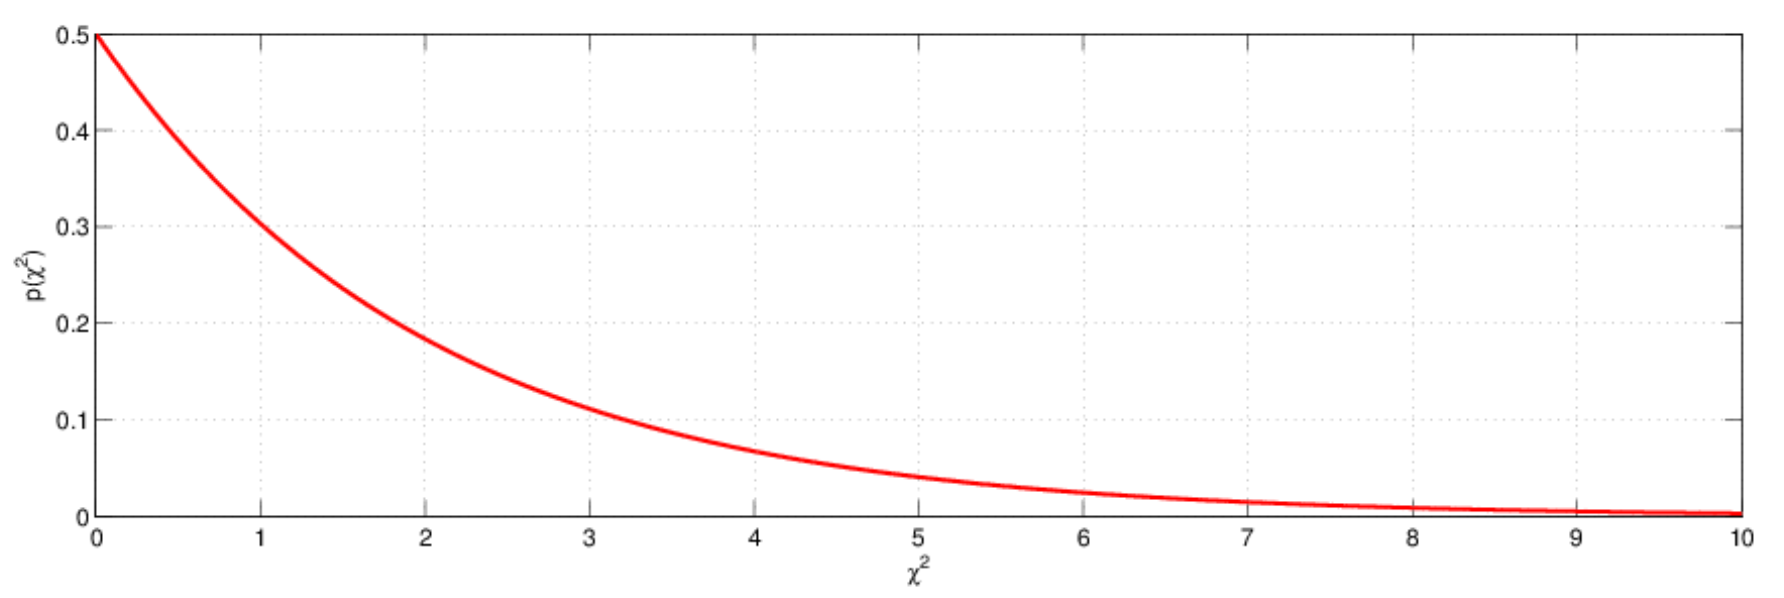
\epsfig{file=figures/jarque_bera.png, scale=0.5}} 
		\caption{Достигаемый уровень значимости}
		\label{target_metric_fig1}
	\end{figure} 

	
	Так как подобные тесты очень чувствительны к выбросам, для проверки используем семплирование и усреднение p-value по семплам. Тест показал, что гипотеза нормальности среднего значения и дисперсии задержек процессов принимается с уровнем значимости $\alpha = 0.05$.
	
	Зная реальное значение целевой переменной и её предсказание, мы можем найти ошибку модели в каждый момент времени - это ещё один временной ряд, который нам необходим для идентификации аномального поведения системы. Масштабирование ошибки необходимо для лучшей  интерпретируемости, в идеале $$0\leq error \leq 1$$
	Но MinMaxScaler не стабилен для данных с выбросами, так как порядок целевой переменной сильно зависит от наличия выбросов в данных, как следствие это влияет на  точность модели, что в свою очередь ведёт к ухудшению интерпретируемости результатов.  Поэтому для оценки качества модели используем более робастный вариант  - масштабирование делением на среднее значение:
	$$error_i =\dfrac{ |a(x_i)-y_i|}{\frac{1}{l}\cdot \sum_i^{l} y_i} $$
	
	Также предложенный  алгоритм поиска аномалий опирается на предположение о нормальности ошибки модели. Проверим эту гипотезу.
\begin{figure}[!htb]
		\minipage{0.49\textwidth}
		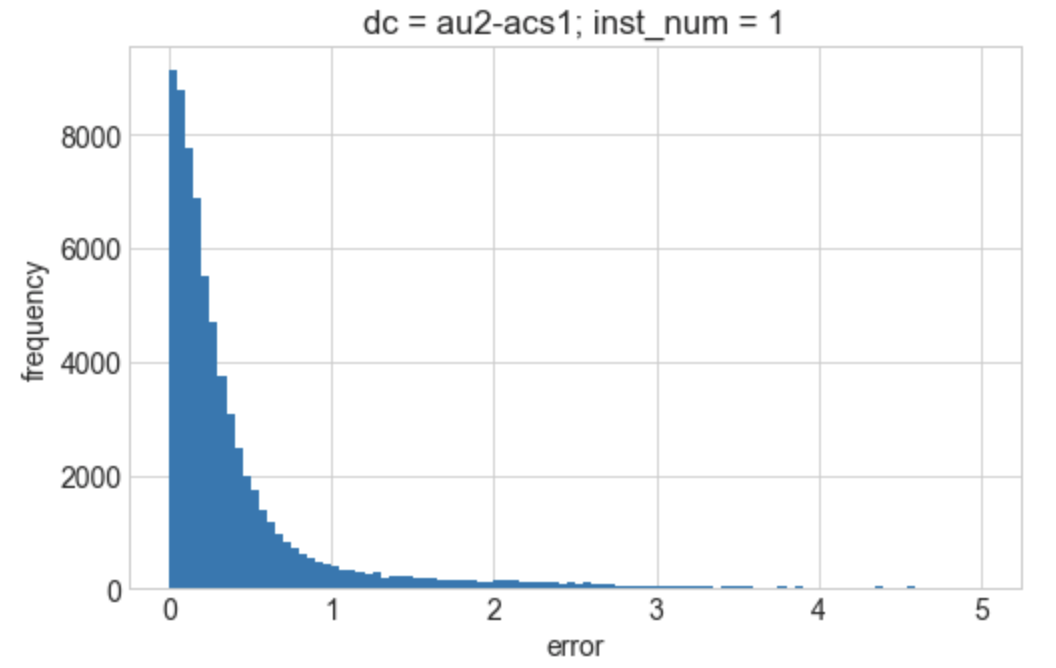
\includegraphics[width=\linewidth]{figures/error_hist.png}
		\caption{dc = au2-acs1; inst = 1}
		\endminipage\hfill
		\minipage{0.49\textwidth}
		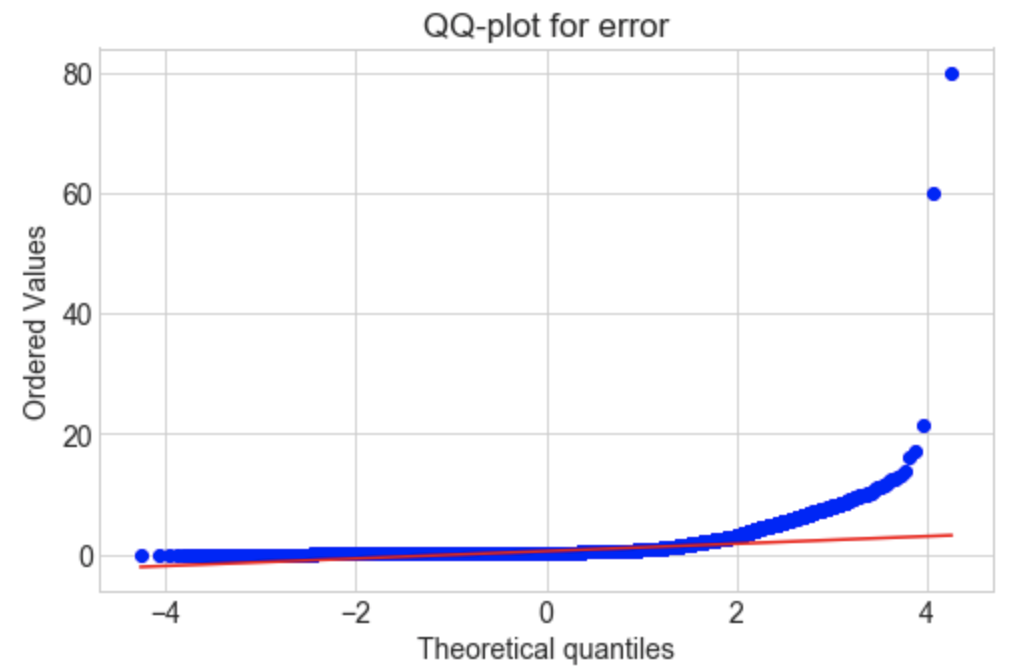
\includegraphics[width=\linewidth]{figures/qq_error.png}
		\caption{dc = au2-acs1; inst = 1}
		\endminipage
	\end{figure}
		
	Аналогичное применение критерия Харке-Бера показало, что гипотеза нормальности ошибки модели принимается с уровнем значимости $\alpha = 0.05$.

	Таким образом мы имеем три нормально распределённые случайные величины для анализа:
	 \begin{enumerate}
	 	\item \texttt{Среднее значение задержек запросов}
	 	\item \texttt{Дисперсия задержек запросов}
	 	\item \texttt{Ошибка модели = отклонение поведения целевой}\\			\texttt{переменной от ожидаемого}
	 \end{enumerate}
	
	Правило трёх сигм - с вероятностью  $0,9973$  значения нормально распределённой случайной величины лежат в интервале $(\mu - 3\sigma,\mu +3 \sigma)$. Мы используем некую вариацию данного правила, используя логичное предположение о том, что нормальное поведение системы находится в зоне высокой вероятности, а аномальное - вне этой зоны. 
	
	То есть будем считать, что нормальное поведение системы находится в интервале $(\mu - k\sigma,\mu +k \sigma)$, где $k$ - гиперпараметр, который мы подберём учитывая мнения экспертов. Очевидно, что значение $k$ зависит от характерной частоты аномального поведения системы и от определения отклонения поведения системы от стандартного. Оба параметра могут быть настроены в соответствии с требованиями заинтересованных сторон.
	
	Будем считать, что характерное количество аномалий на некотором хранилище данных за $D$ дней задаётся следующей формулой:
	$$ n = \dfrac{N_{dc}\cdot \nu \cdot D}{N}$$
	$N_{dc}$ - количество загруженных экземпляров данного хранилища данных 
	$N = 30 $ - максимальное количество экземпляров хранилища данных \\
	$\nu$ - характерная частота аномального поведения системы 

	Дальнейшие вычисления приведены в предположении, что  $\nu= \frac{20}{30}$ и $D = 60$. То есть мы предполагаем, что для системы характерно иметь 40 аномалий за 60 дней на полностью загруженном хранилище данных.
	
	Таким образом мы имеем три метрики и решающее правило для поиска аномального поведения. Применение к любой метрике  решающего правила позволяет разделить входные данные на две группы - моменты аномального и нормального поведения системы. Наша модель должна удовлетворять требованиям заинтересованных сторон, по мнению которых аномальное поведение системы зачастую длится больше минуты. Поэтому аномальные моменты времени необходимо кластеризовать в аномальные интервалы времени, длительностью  больше одной минуты.
	
	Применим следующий алгоритм:
	\begin{enumerate}
	 	\item \texttt{С помощью метрики и решающего правила разделим входные данные на две группы - моменты аномального и нормального поведения\\ системы.}
	 	\begin{figure}[H]
		\centerline{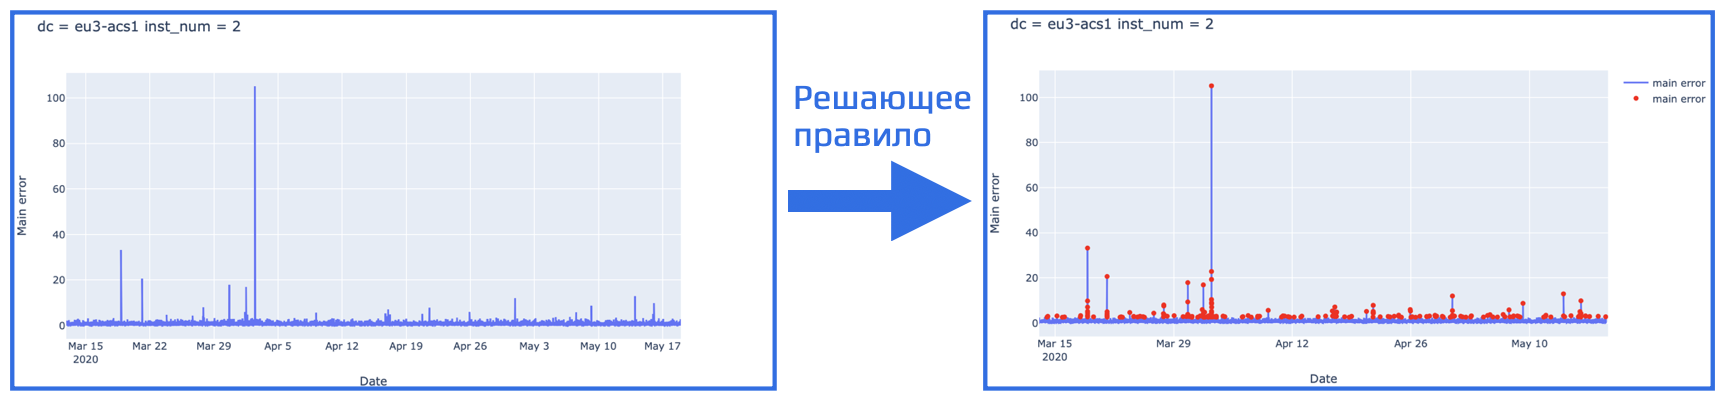
\epsfig{file=figures/apply_sigma_rule.png, scale=0.55}} 
		\caption{Применение решающего правила к ошибке модели}
		\label{target_metric_fig1}
	\end{figure} 
	\item \texttt{Для каждой аномальной точки рассмотрим окно в T минут. Если \\внутри такого окна аномальных моментов времени больше, чем n, то интервал между рассматриваемой аномальной точкой и последней аномальной точкой в окне помечается, как аномальный.}
	\begin{figure}[H]
		\centerline{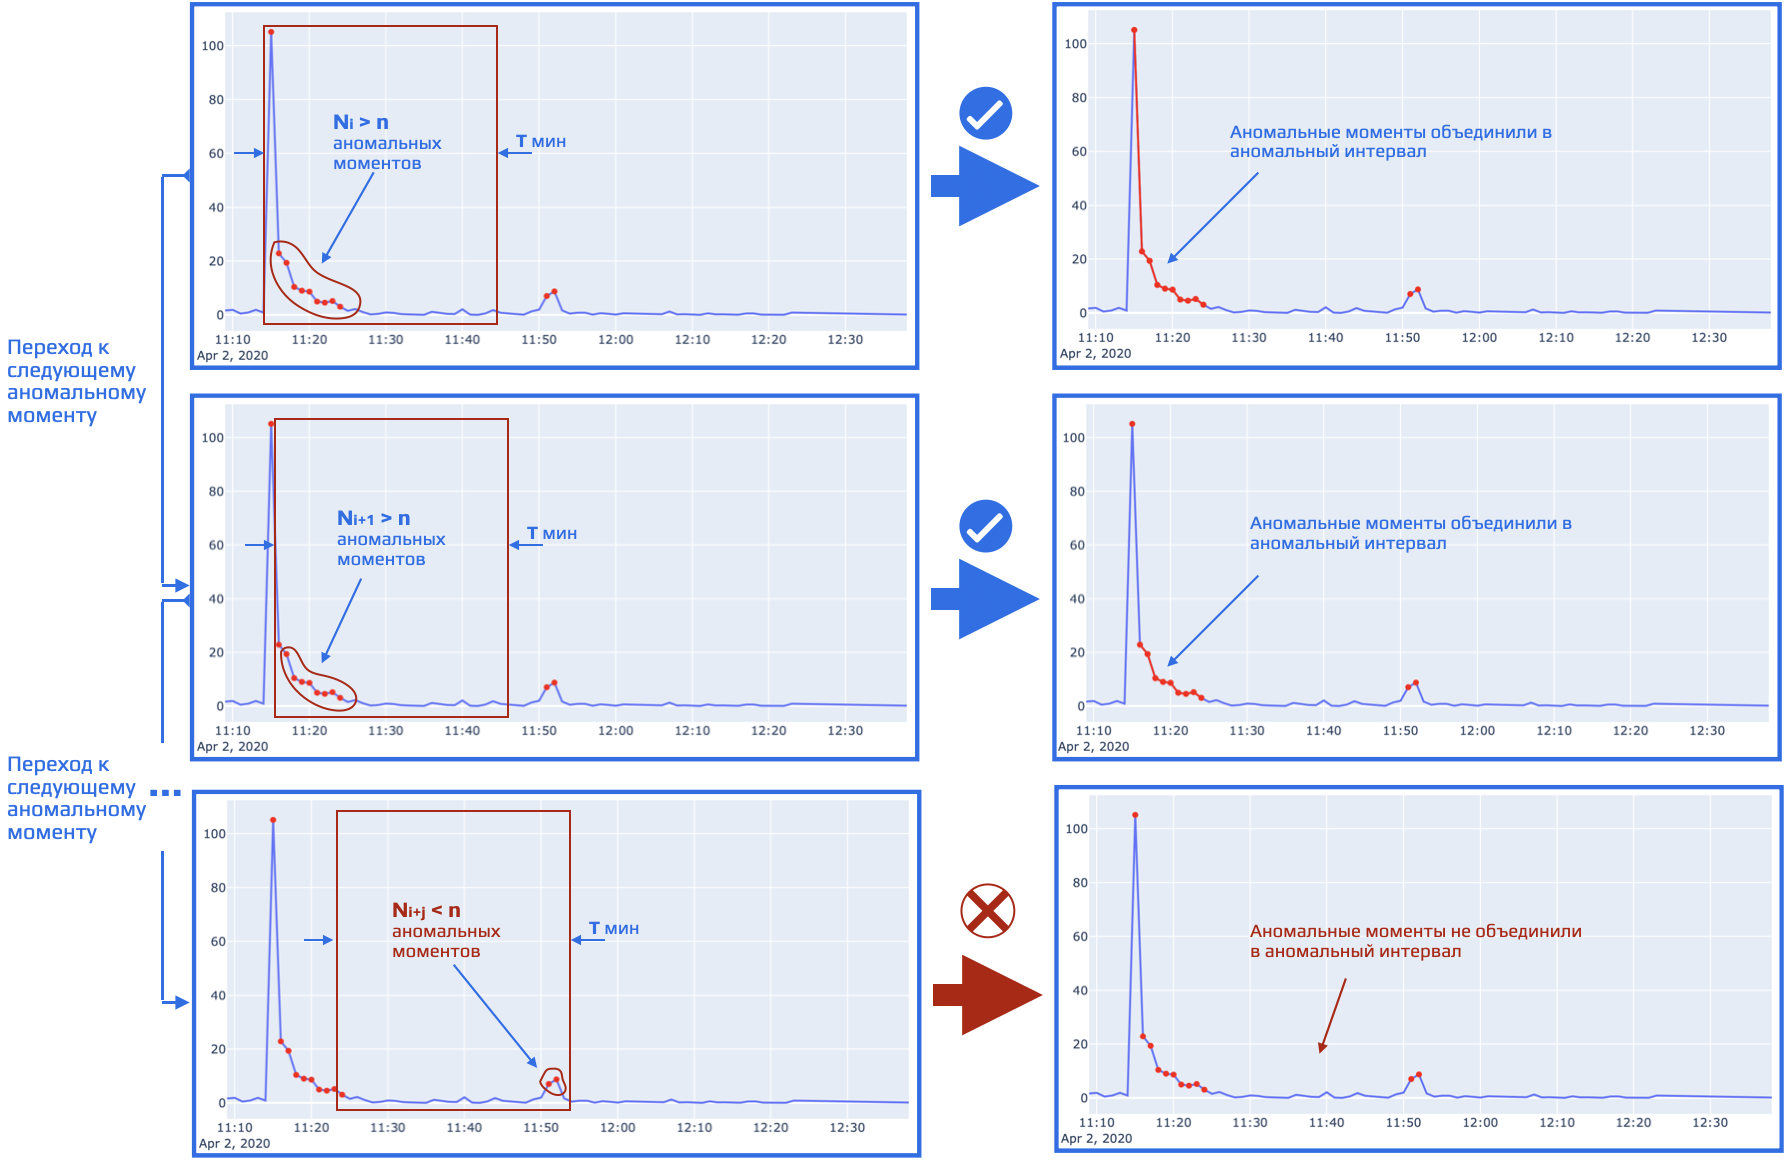
\epsfig{file=figures/all_proces.png, scale=0.55}} 
		\caption{Процедура построения аномальных интервалов}
		\label{target_metric_fig1}
	\end{figure} 
	\item \texttt{Далее все пересекающиеся аномальные интервалы объединяются.}	
	\begin{figure}[H]
		\centerline{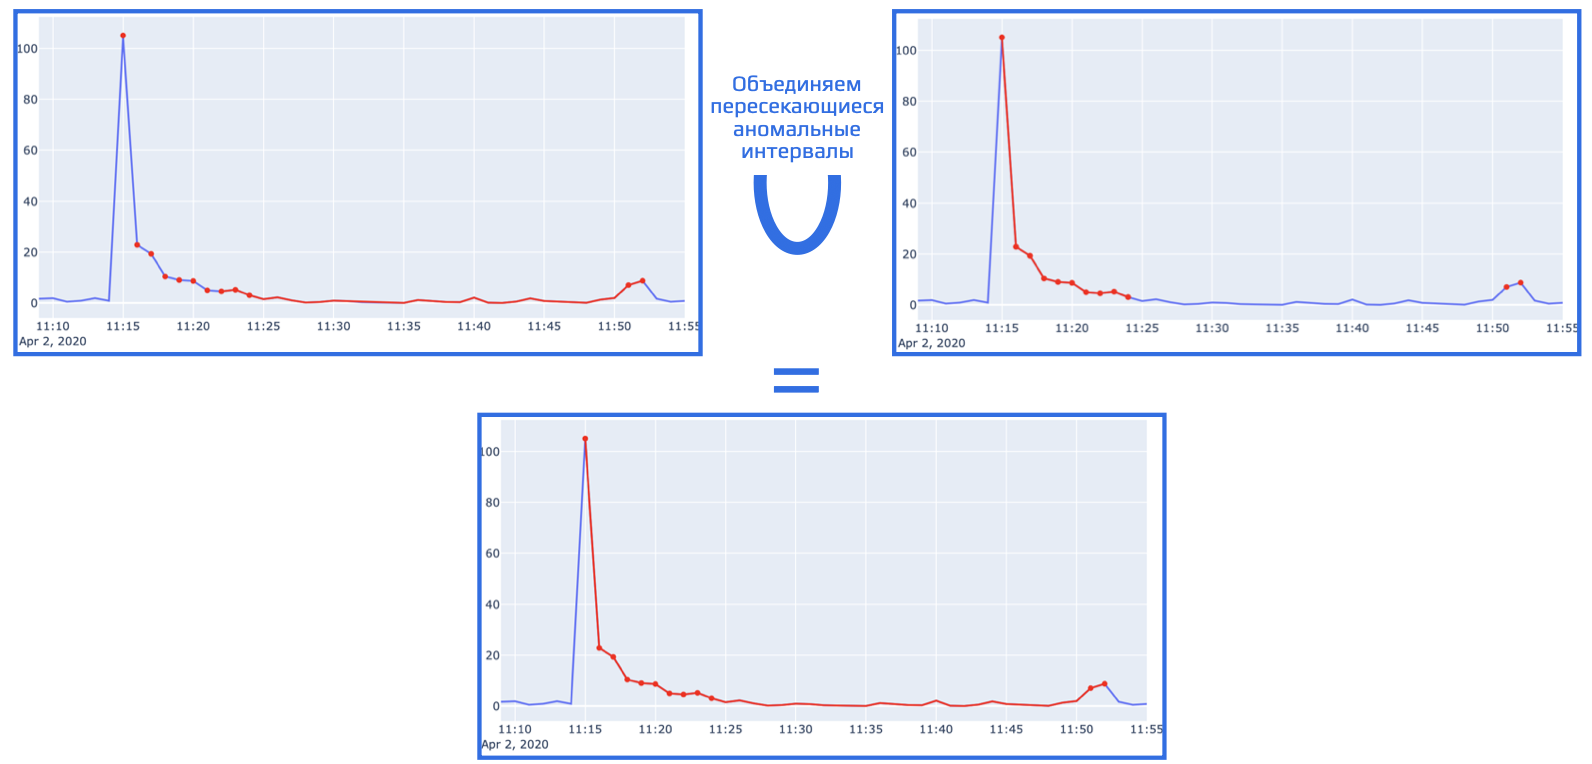
\epsfig{file=figures/union_process.png, scale=0.6}} 
		\caption{Процедура объединения аномальных интервалов}
		\label{target_metric_fig1}
	\end{figure} 
	\end{enumerate}
	
	Таким образом для рассматриваемой метрики мы получаем аномальные интервалы времени:
	\begin{figure}[H]
		\centerline{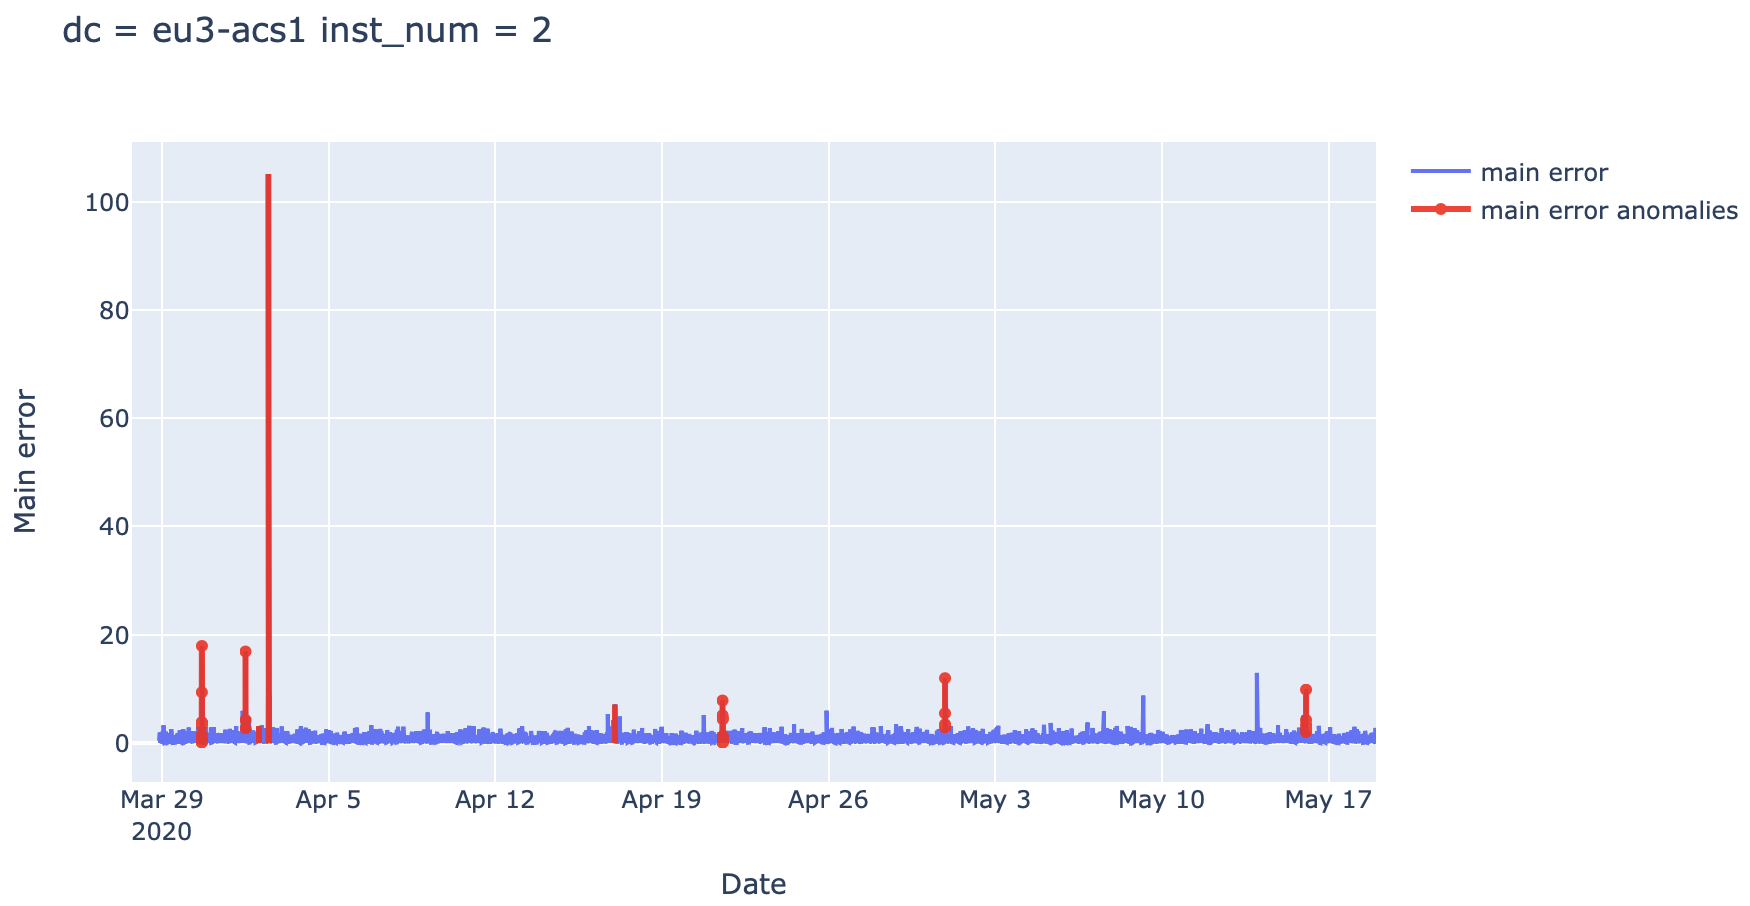
\epsfig{file=figures/example_of_anomaly_interval_error.png, scale=0.50}} 
		\caption{Итог алгоритма поиска аномальных интервалов по соответствующей метрике}
		\label{target_metric_fig1}
	\end{figure} 
	
	Выберем наиболее информативную метрику для детектирования аномалий. Для этого рассмотрим зависимость количества аномальных интервалов от числа $k$ для имеющихся у нас нормальных случайных величин, характеризующих поведение системы. 
	\begin{figure}[!htb]
		\minipage{0.52\textwidth}
		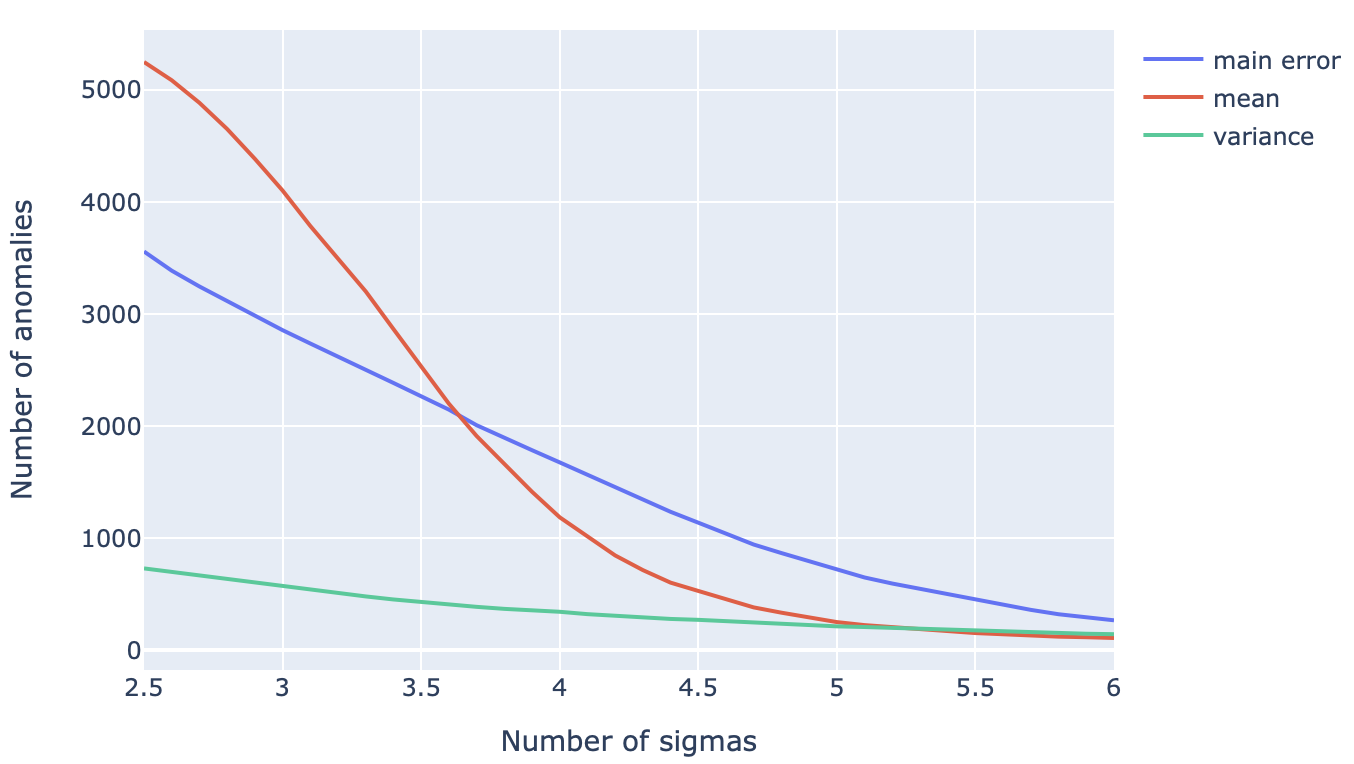
\includegraphics[width=\linewidth]{figures/modes_au2_acs1.png}
		\caption{dc = au2-acs1}
		\endminipage\hfill
		\minipage{0.52\textwidth}
		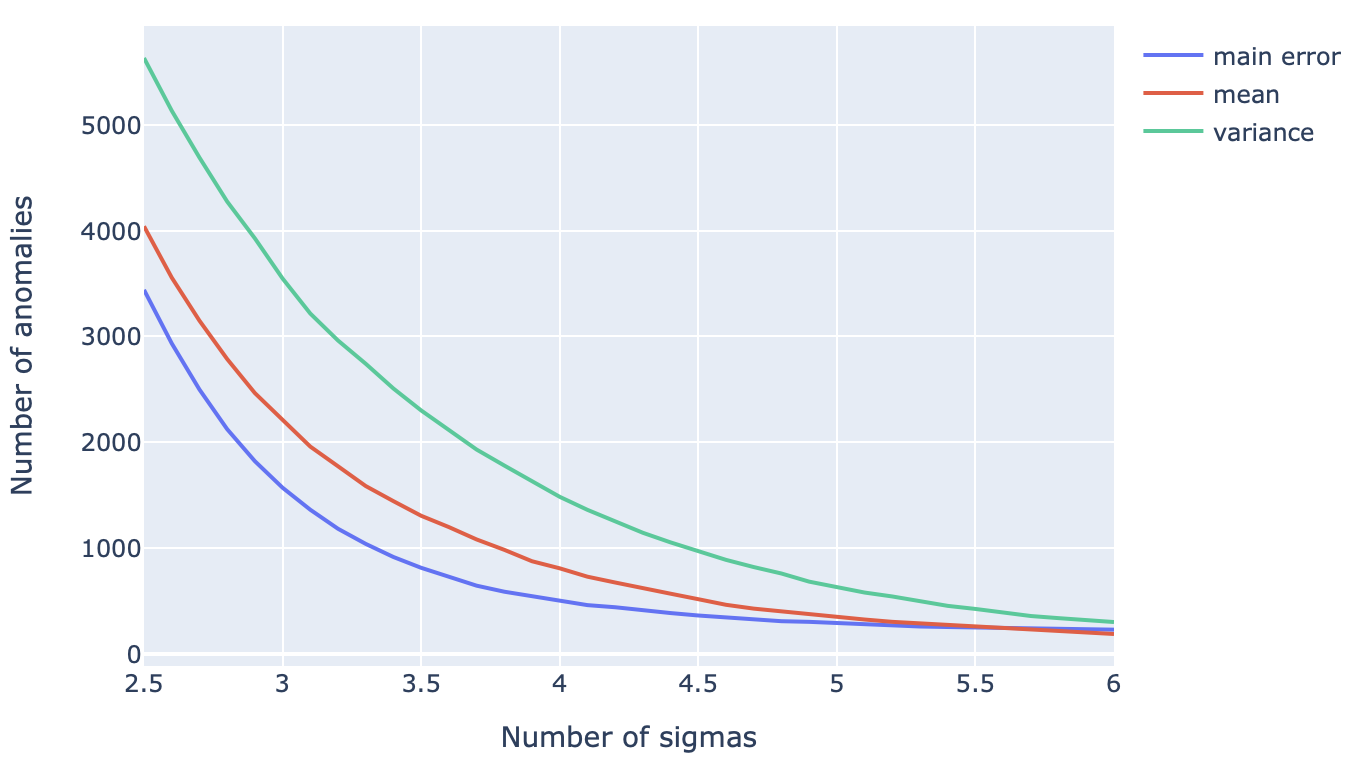
\includegraphics[width=\linewidth]{figures/modes_eu3_acs1.png}
		\caption{dc = eu3-acs1}
		\endminipage
	
		\minipage{0.52\textwidth}
		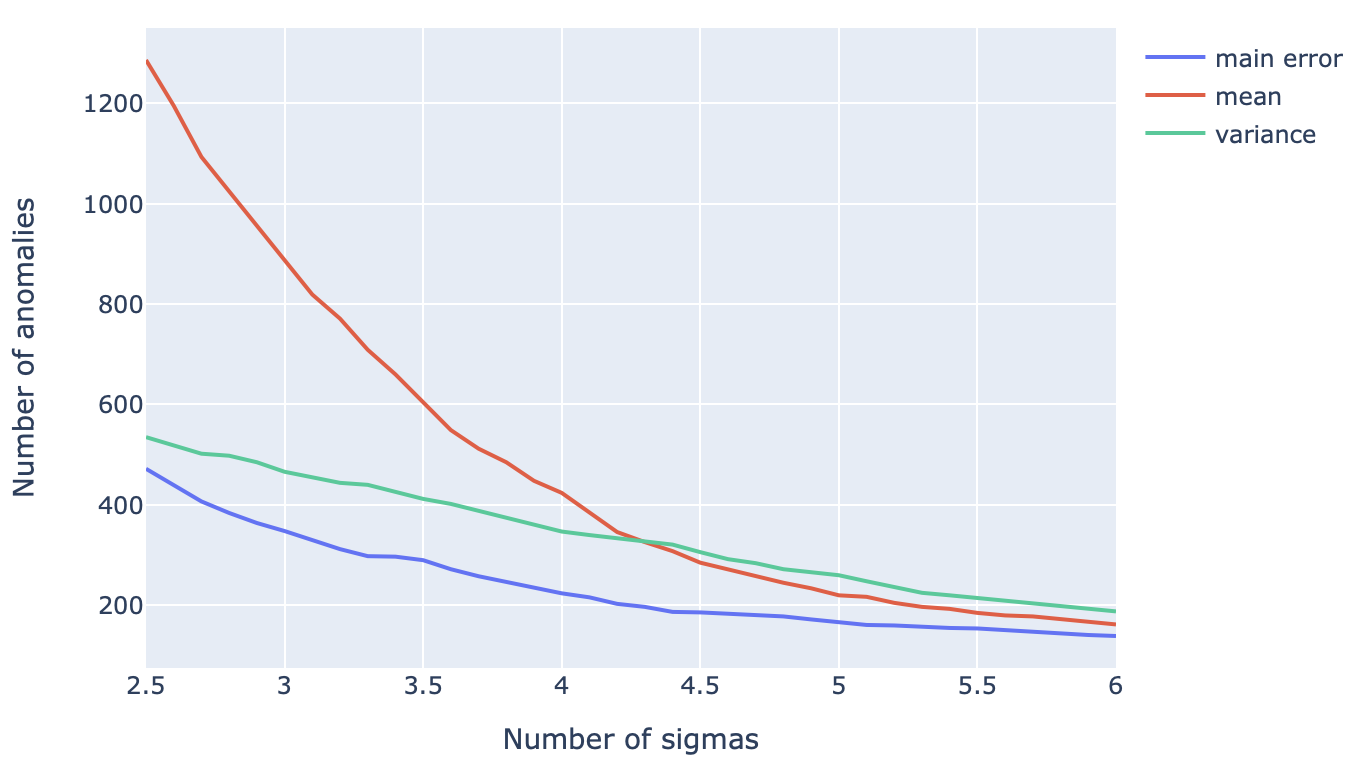
\includegraphics[width=\linewidth]{figures/modes_us3.png}
		\caption{dc = us3}
		\endminipage\hfill
		\minipage{0.52\textwidth}
		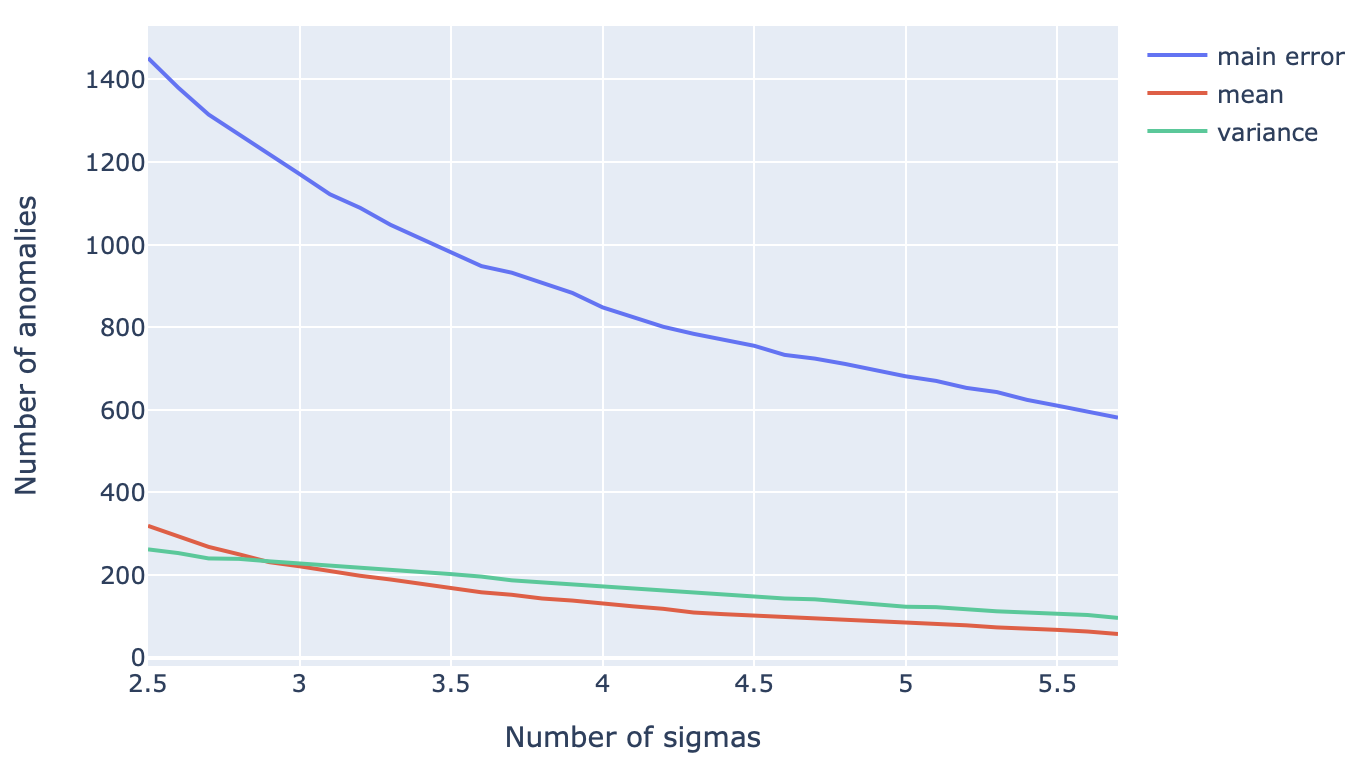
\includegraphics[width=\linewidth]{figures/modes_us6_acs2.png}
		\caption{dc = us6-acs2}
		\endminipage
	\end{figure}
	
	Логично предположить, что во время аномального поведения системы сразу несколько из этих параметров должны отклонятся от стандартного поведения. То есть аномальные интервалы, вычисленные по разным метрикам, должны совпадать, ну или, по крайней мере, пересекаться. 
	
	Судя по графикам, дисперсия задержек не является  универсальной метрикой для поиска аномалий, так как её поведение сильно отличается на разных хранилищах данных. Поэтому рассмотрим сложносоставную метрику - "$\texttt{логическое И}$" \;результатов поиска аномалий по двум оставшимся метрикам. Таким образом аномальными интервалами будем считать все непустые пересечения аномальных интервалов, найденных с помощью среднего значения  задержек процессов и ошибки модели.
	\begin{figure}[H]
		\centerline{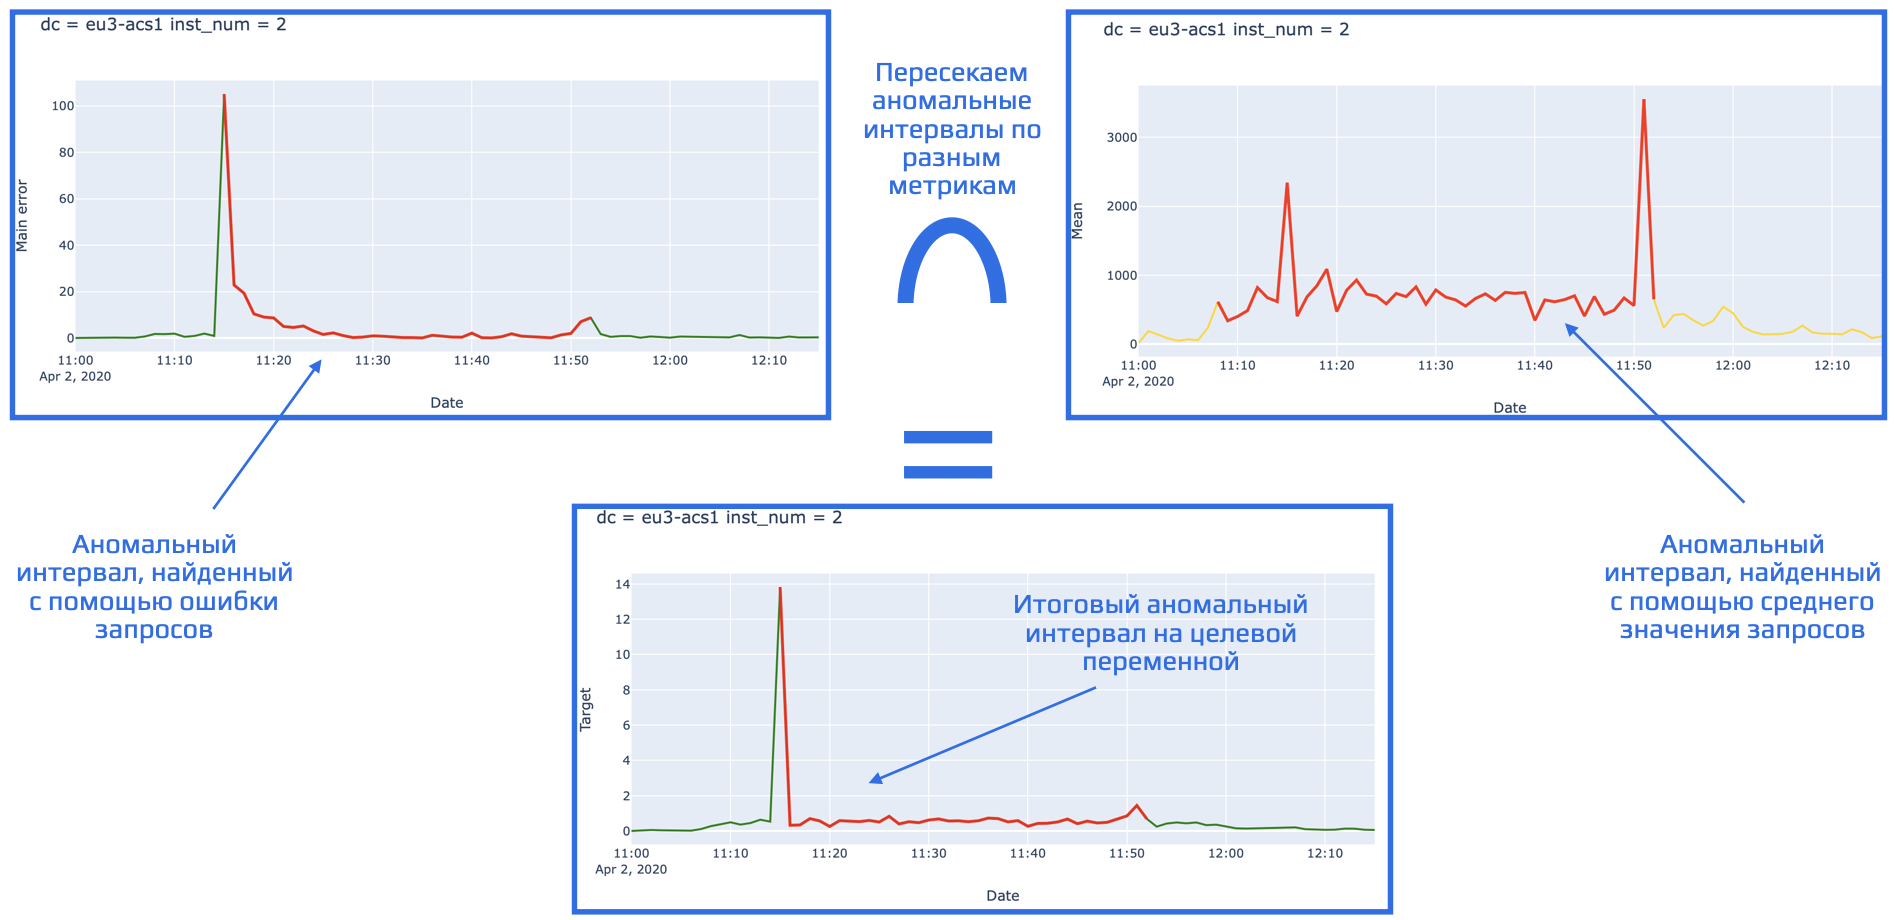
\epsfig{file=figures/intersection_process.png, scale=0.5}} 
		\caption{Сложносоставная метрика}
		\label{target_metric_fig1}
	\end{figure} 
	С помощью этой метрики подберём параметр $k$ и протестируем наш алгоритм. 
	
	
	\section{Результаты работы алгоритма}	
	\begin{figure}[H]
		\centerline{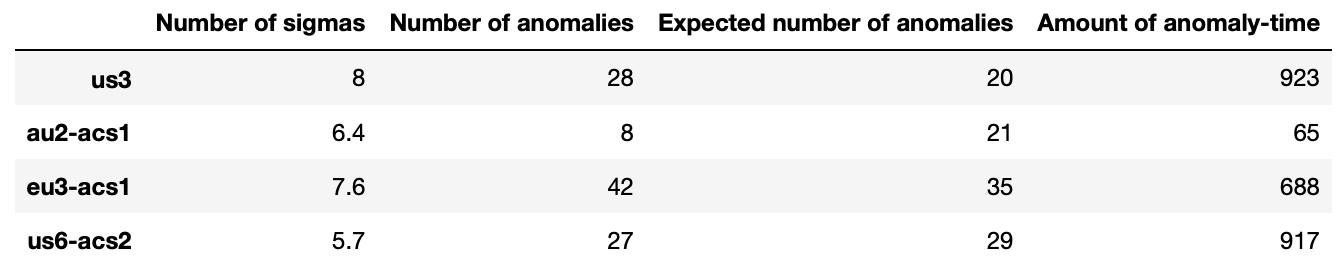
\epsfig{file=figures/result_table.png, scale=0.70}} 
		\caption{Сводная таблица результатов работы алгоритма}
		\label{target_metric_fig1}
	\end{figure} 
	\begin{figure}[H]
		\centerline{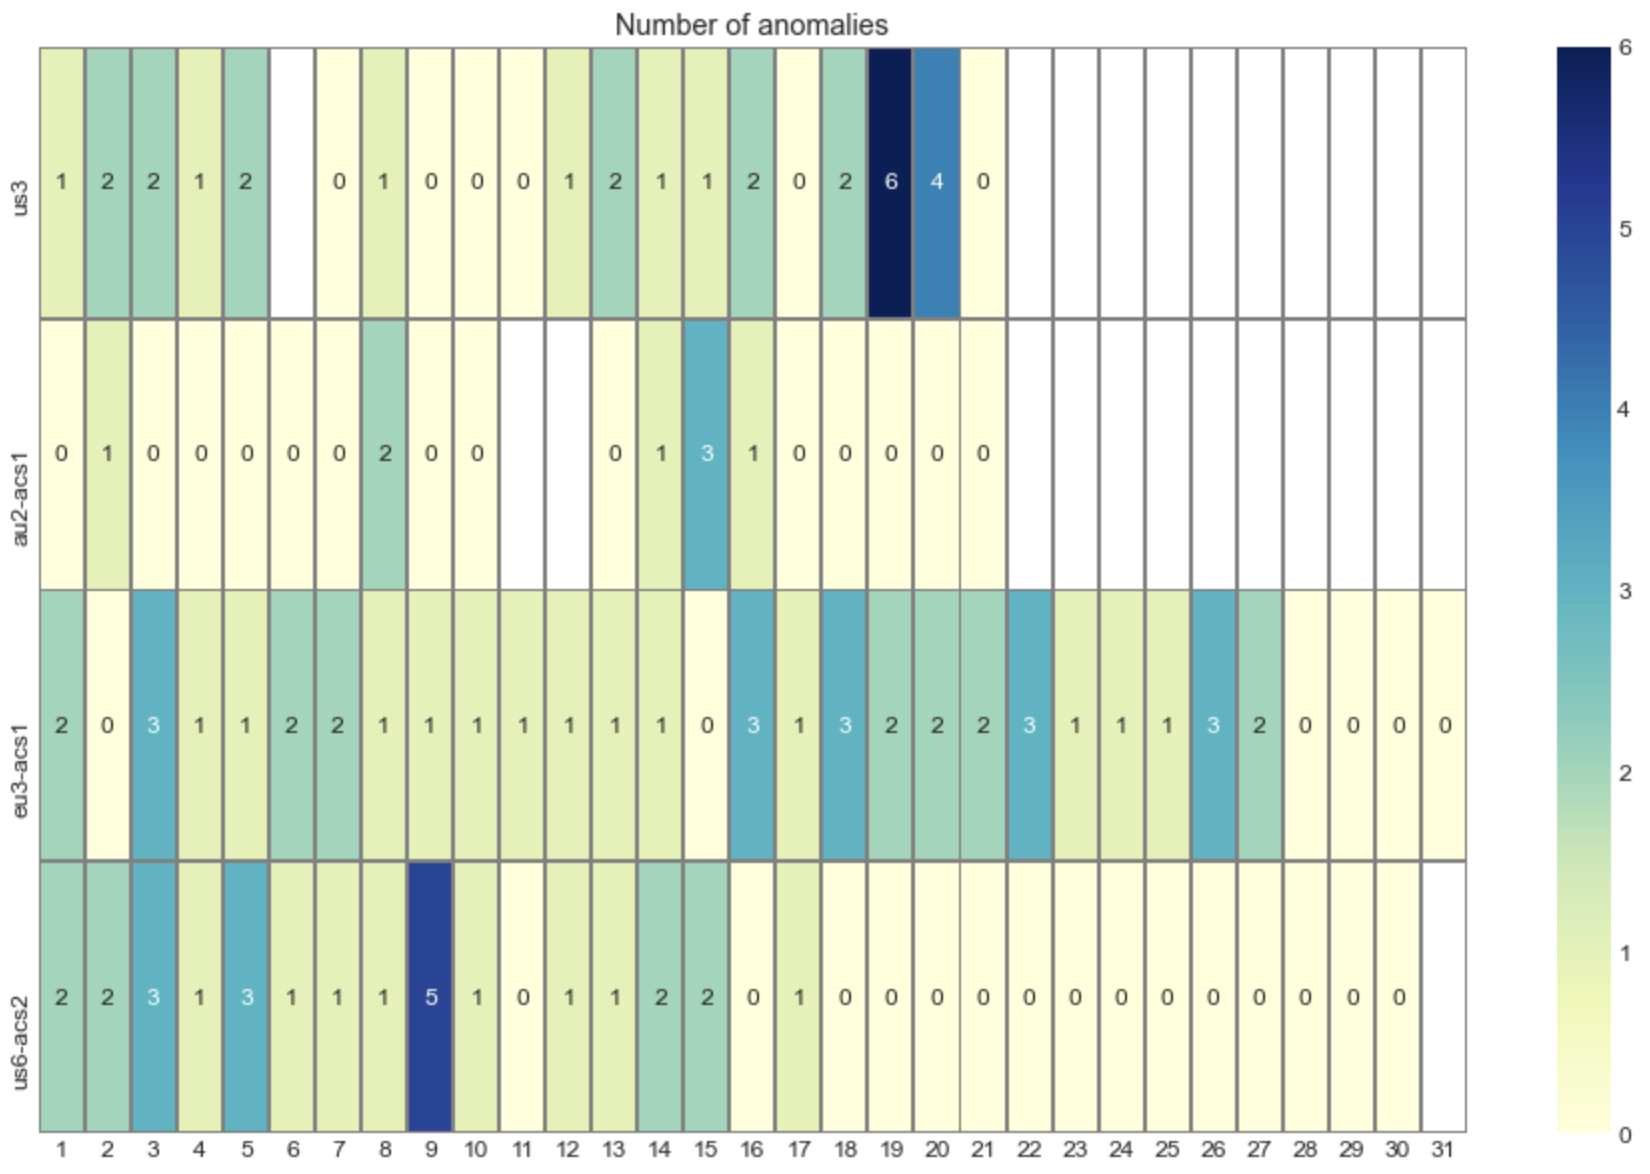
\epsfig{file=figures/heat_map_number.png, scale=0.5}} 
		\caption{Тепловая карта количества аномалий}
		\label{target_metric_fig1}
	\end{figure} 
	\begin{figure}[H]
		\centerline{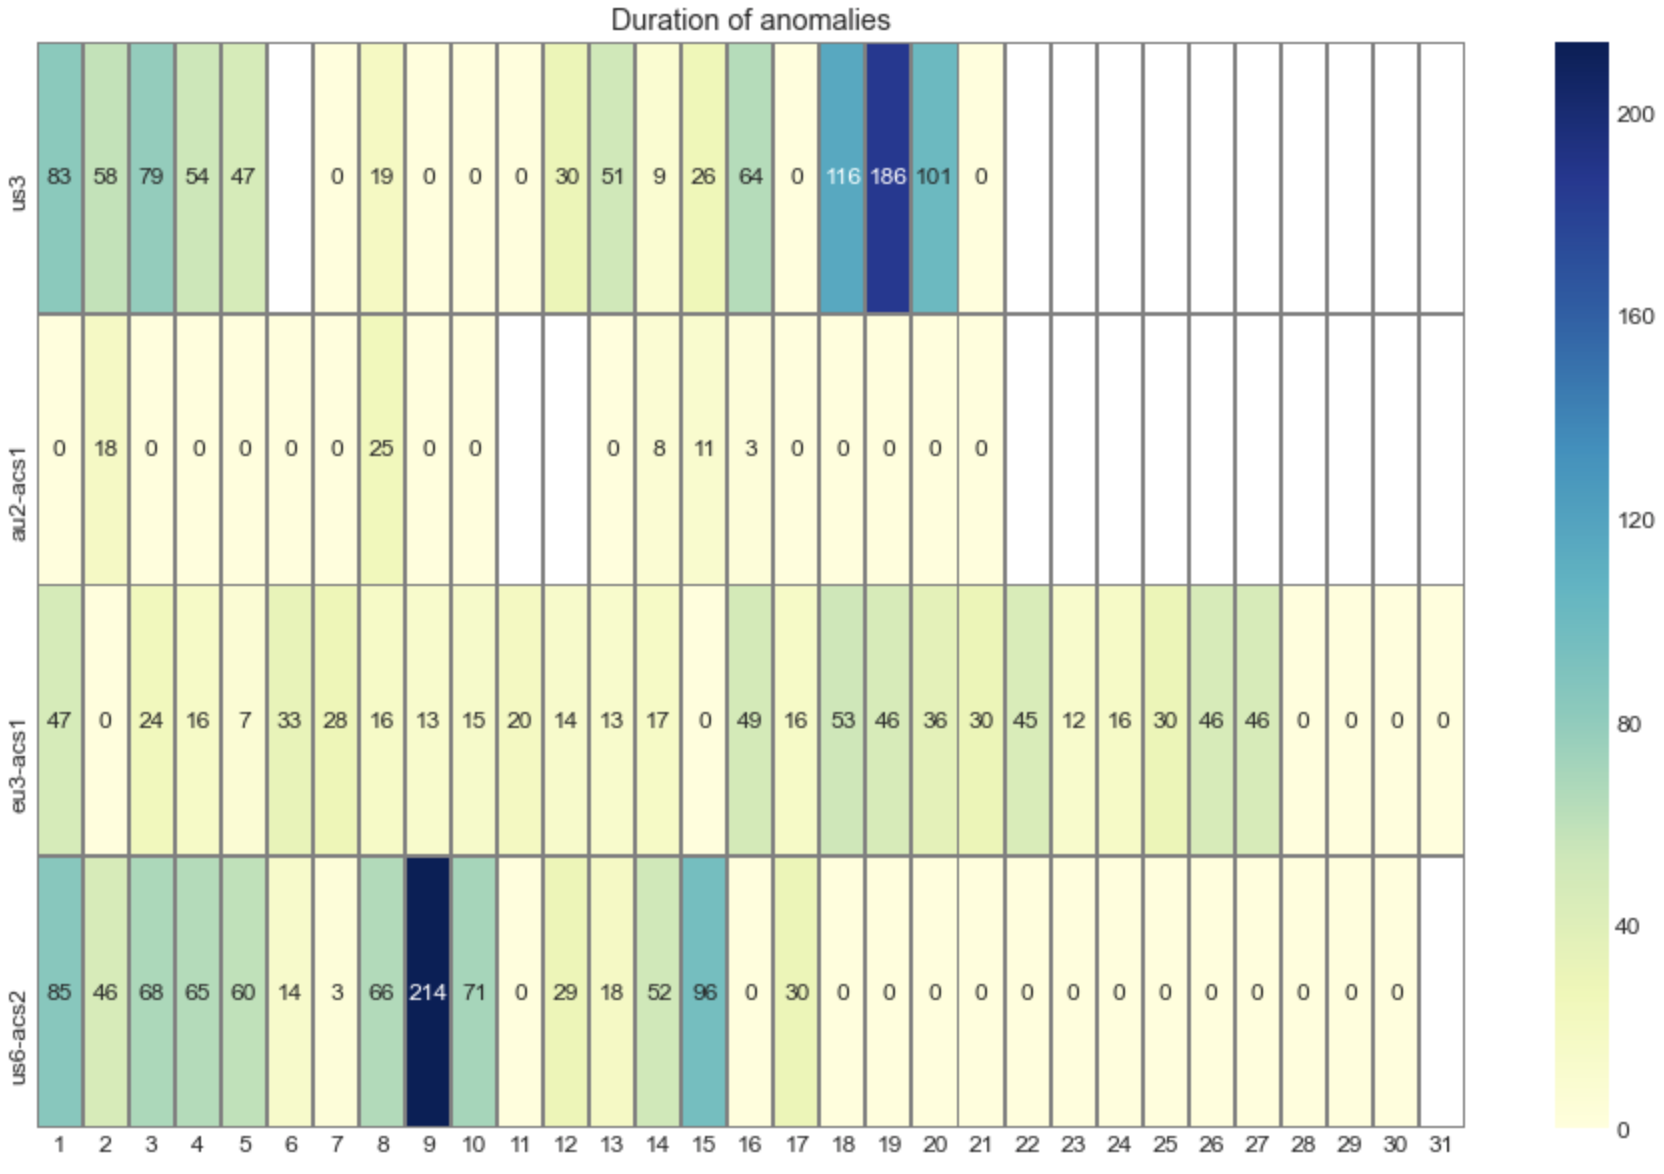
\epsfig{file=figures/heat_map_duration.png, scale=0.50}} 
		\caption{Тепловая карта суммарной длительности аномалий в минутах}
		\label{target_metric_fig1}
	\end{figure} 

	 \section{Примеры найденных аномалий}	
\begin{figure}[H]
		\centerline{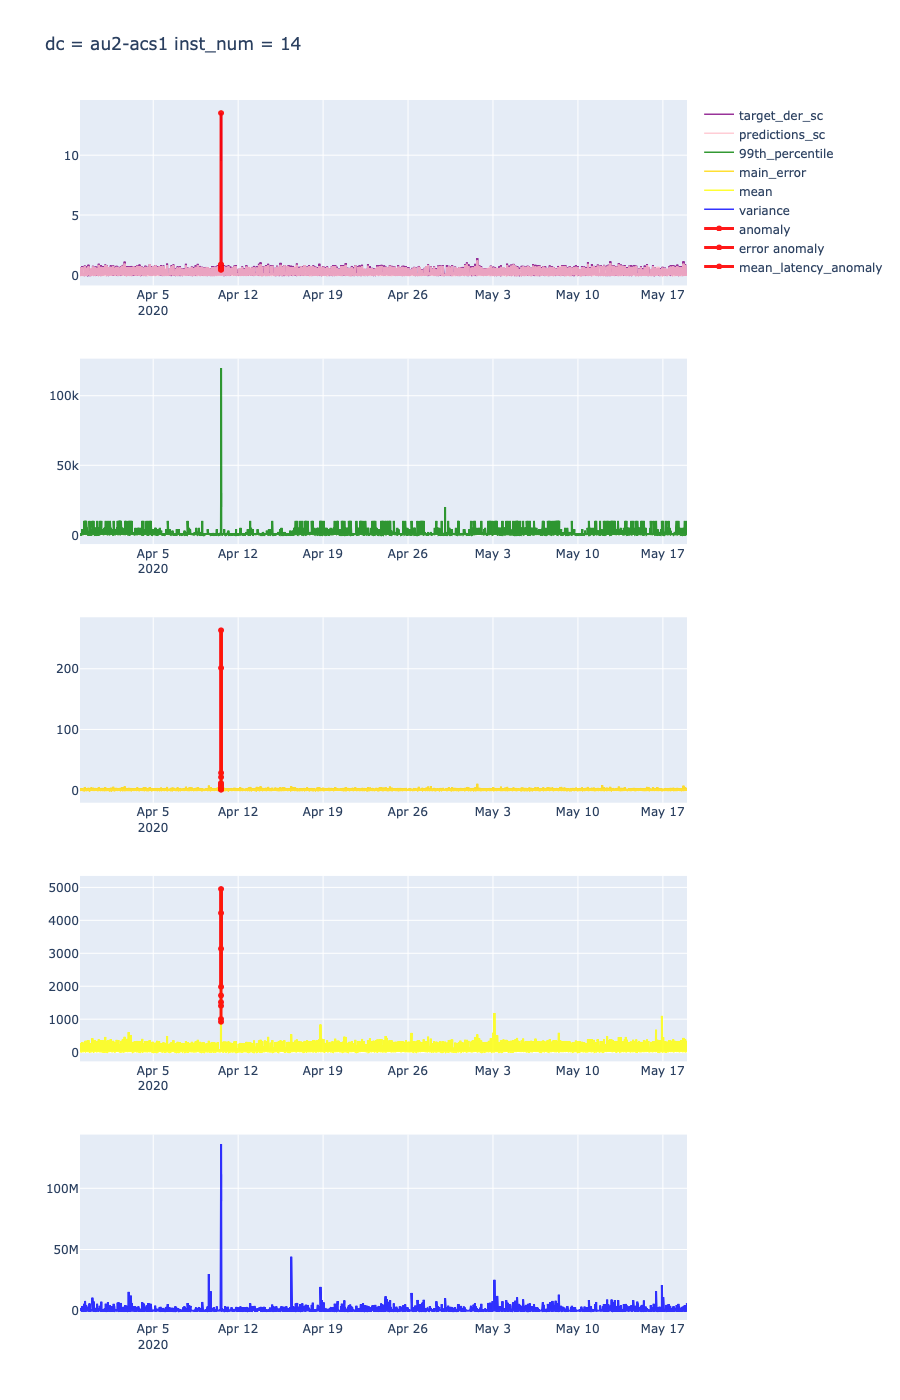
\epsfig{file=figures/full_example1.png, scale=0.47}} 
		\caption{Пример найденной аномалии}
		\label{target_metric_fig1}
	\end{figure} 
	
	\section{Проверка корректности алгоритма}	
 По мнению экспертов, аномальное поведение системы зачастую сопровождается резким увеличением $99$-го персентиля задержки запросов. Проверим корректность алгоритма следующим образом: если найденная аномалия сопровождается ростом $99$-го персентиля задержки запросов, то считаем, что алгоритм сработал верно, иначе считаем, что алгоритм сработал неверно. 
	\begin{figure}[H]
		\centerline{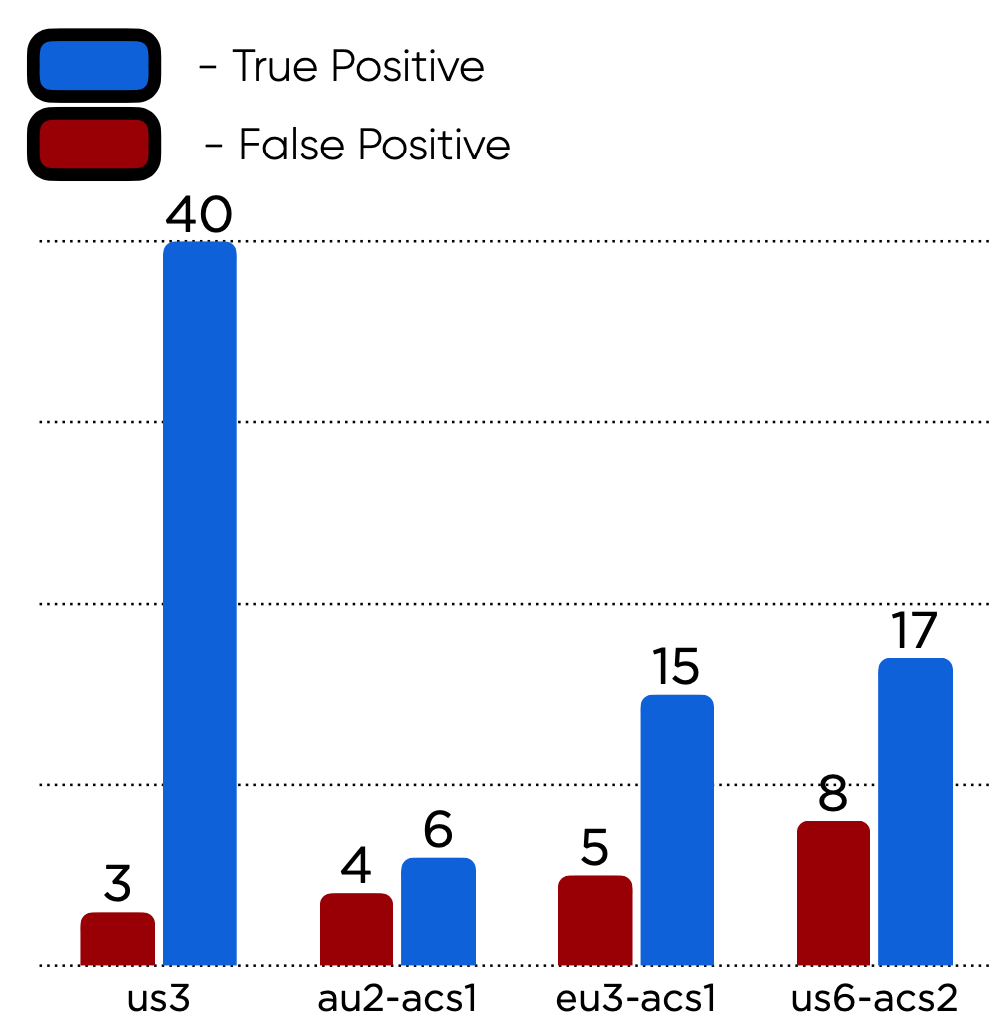
\epsfig{file=figures/conf_matrix.png, scale=0.70}} 
		\caption{Корректность алгоритма}
		\label{target_metric_fig1}
	\end{figure} 
	Таким образом точность алгоритма: 
	$$\textbf{accuracy = 82\%}$$
	\newpage
	\section{Заключение}	
	В результате работы была создан универсальный для всего  многообразия хранилищ данных компании Acronis алгоритм детектирования аномалий, имеющий высокую точность.
	\\\\
	 Преимуществами алгоритма являются: 
	  \begin{enumerate}
	 	\item \texttt{Полное отсутсвие ручной работы.}
	 	\item \texttt{Универсальность для всего многообразия хранилищ данных \\компании Acronis.}
	 	\item \texttt{Легко настраивается под требования заинтересованных сторон.}
	 	\item \texttt{Одинаково корректная работа при любой нагрузке системы.}
	 	\item \texttt{Высокая точность.}
		\item \texttt{Низкий уровень ложных срабатываний.}
\end{enumerate}

	 Выявление аномального поведения в автоматическом режиме позволит повысить  качество работы системы Acronis Storage, а также поможет предотвращать нештатные ситуации на этапах их зарождения. 
	
	Логическим продолжением этой работы является использование алгоритма для разметки исторических данных, которая необходима для построения  модели заблаговременного предсказания аномального поведения системы. 
	
	
	
	
	
	\newpage
	\begin{thebibliography}{228}
		\bibitem{cite1} 
		\emph{Prometheus - an open-source systems monitoring and alerting toolkit.} 
		URL: https://prometheus.io/.
		\bibitem{cite2} 
		\emph{G. E. P. Box, G. M. Jenkins, and G. C. Reinsel.} 
		Time Series Analysis: Forecasting and Control, John Wiley $\&$ Sons, New York, NY, USA, 2013.
		\bibitem{cite3} 
		\emph{Arindam Banerjee Varun Chandola and Vipin Kumar.} 
		Anomaly detection : A survey, ACM Computing Surveys, 2009. 
		\bibitem{cite4} 
		\emph{Dominique T. Shipmon, Jason M. Gurevitch, Paolo M. Piselli, Steve Edwards.} 
		Detection of Anomalous Drops with Limited Features and Sparse Examples in Noisy Highly Periodic Data. 
		\bibitem{cite5} 
		\emph{Ane Blazquez-Garcia and Angel Conde.} 
		A review on outlier/anomaly detection in time series data.
	\end{thebibliography}
			
\end{document}
				
				
				
